\documentclass[12pt,aspectratio=169]{beamer}

\usetheme[progressbar=frametitle]{metropolis}
\usepackage{appendixnumberbeamer}

\usepackage{booktabs}
\usepackage[scale=2]{ccicons}

\usepackage{pgfplots}
\usepgfplotslibrary{dateplot}

\usepackage{xspace}
\newcommand{\themename}{\textbf{\textsc{metropolis}}\xspace}

\usepackage{datetime}

\usepackage{threeparttable}
\usepackage{multirow}
\usepackage{tabularx}
\usepackage[]{siunitx}
\usepackage{makecell}
\usepackage{diagbox}
\usepackage[absolute,overlay]{textpos}
\usepackage{etoolbox}
%\usepackage{setspace}

% Grid
%\usepackage[texcoord,grid,gridunit=mm,gridcolor=red!10,subgridcolor=green!10]{eso-pic}


\usepackage{pifont}
\newcommand{\cmark}{\textcolor{green!50!white}{\ding{51}}}%
\newcommand{\xmark}{\textcolor{red!50!white}{\ding{55}}}%
\newcommand{\eqmark}{{\bf \(\approx\)}}

\definecolor{lightgray}{rgb}{0.83, 0.83, 0.83}
\definecolor{lightblue}{rgb}{0.68, 0.85, 0.9}
\definecolor{lightgreen}{rgb}{0.56, 0.93, 0.56}
\definecolor{thistle}{rgb}{0.85, 0.75, 0.85}

\setbeamerfont{subsection in toc}{size=\scriptsize}

%\makeatletter
%\patchcmd{\beamer@sectionintoc}{\vskip1.5em}{\vskip0.5em}{}{}
%\makeatother

\usepackage{soul}
%\sethlcolor{yellow!60!white}

\makeatletter
\let\HL\hl
\renewcommand\hl{%
  \let\set@color\beamerorig@set@color
  \let\reset@color\beamerorig@reset@color
  \HL}
\makeatother

\usepackage{minted}
\setminted{fontsize=\scriptsize}

\newdate{dateSoutenance}{04}{11}{2022}


\usepackage[backend=biber,
            defernumbers=true,
            sorting=ynt,
            %style=numeric,
            style=authortitle,
            %style=draft,
            backref=true]{biblatex}
\addbibresource{../bibliography.bib}


\title{Generic programming in modern C++ for\\ Image Processing}
%\subtitle{}
\date{Thesis Defense --- \displaydate{dateSoutenance}}
\author{\textbf{Michaël Roynard} \hspace{1cm} Director: \emph{Thierry Géraud} \hspace{1cm} Supervisor: \emph{Edwin Carlinet}}
\institute{EPITA Research Laboratory (LRE) --- Le Kremlin-Bicêtre, France}
\titlegraphic{

\includegraphics[width=.2\textwidth]{../images/logo-edite}\hfill

\includegraphics[width=.2\textwidth]{../images/epita}\hfill

\includegraphics[width=.2\textwidth]{../images/lre-logo.png}\hfill

\includegraphics[width=.2\textwidth]{../images/Logo_of_Sorbonne_University}
}

\makeatletter
\setbeamertemplate{title page}{
  \begin{minipage}[b][\paperheight]{\textwidth}
    \vfill%
    \ifx\inserttitle\@empty\else\usebeamertemplate*{title}\fi
    \ifx\insertsubtitle\@empty\else\usebeamertemplate*{subtitle}\fi
    \usebeamertemplate*{title separator}
    \ifx\beamer@shortauthor\@empty\else\usebeamertemplate*{author}\fi
    \ifx\insertdate\@empty\else\usebeamertemplate*{date}\fi
    \ifx\insertinstitute\@empty\else\usebeamertemplate*{institute}\fi
    \vfill
    \ifx\inserttitlegraphic\@empty\else\inserttitlegraphic\fi
    \vspace*{1cm}
  \end{minipage}
}
\makeatother

\begin{document}

\maketitle

\begin{frame}{Overview}
  \setbeamertemplate{section in toc}[sections numbered]
  %\singlespacing
  \tableofcontents[hideallsubsections]
\end{frame}

%
%
%

\section[General introduction]{General introduction}

\begin{frame}[fragile]{Image processing nowadays}
  \begin{itemize}
    \item Image processing is everywhere, in most of the devices (computer, phone, embedded devices, etc.)
    \item Applications are multiples (medical imaging, social network filters, facial recognition, etc.).
    \item Every industry and research domain is using it (production line automation, automatic document reading, social network apps, etc.)
    \item Image Processing is costly in resources. Performance is crucial.
  \end{itemize}
  \begin{figure}[bl]
    \hfill
    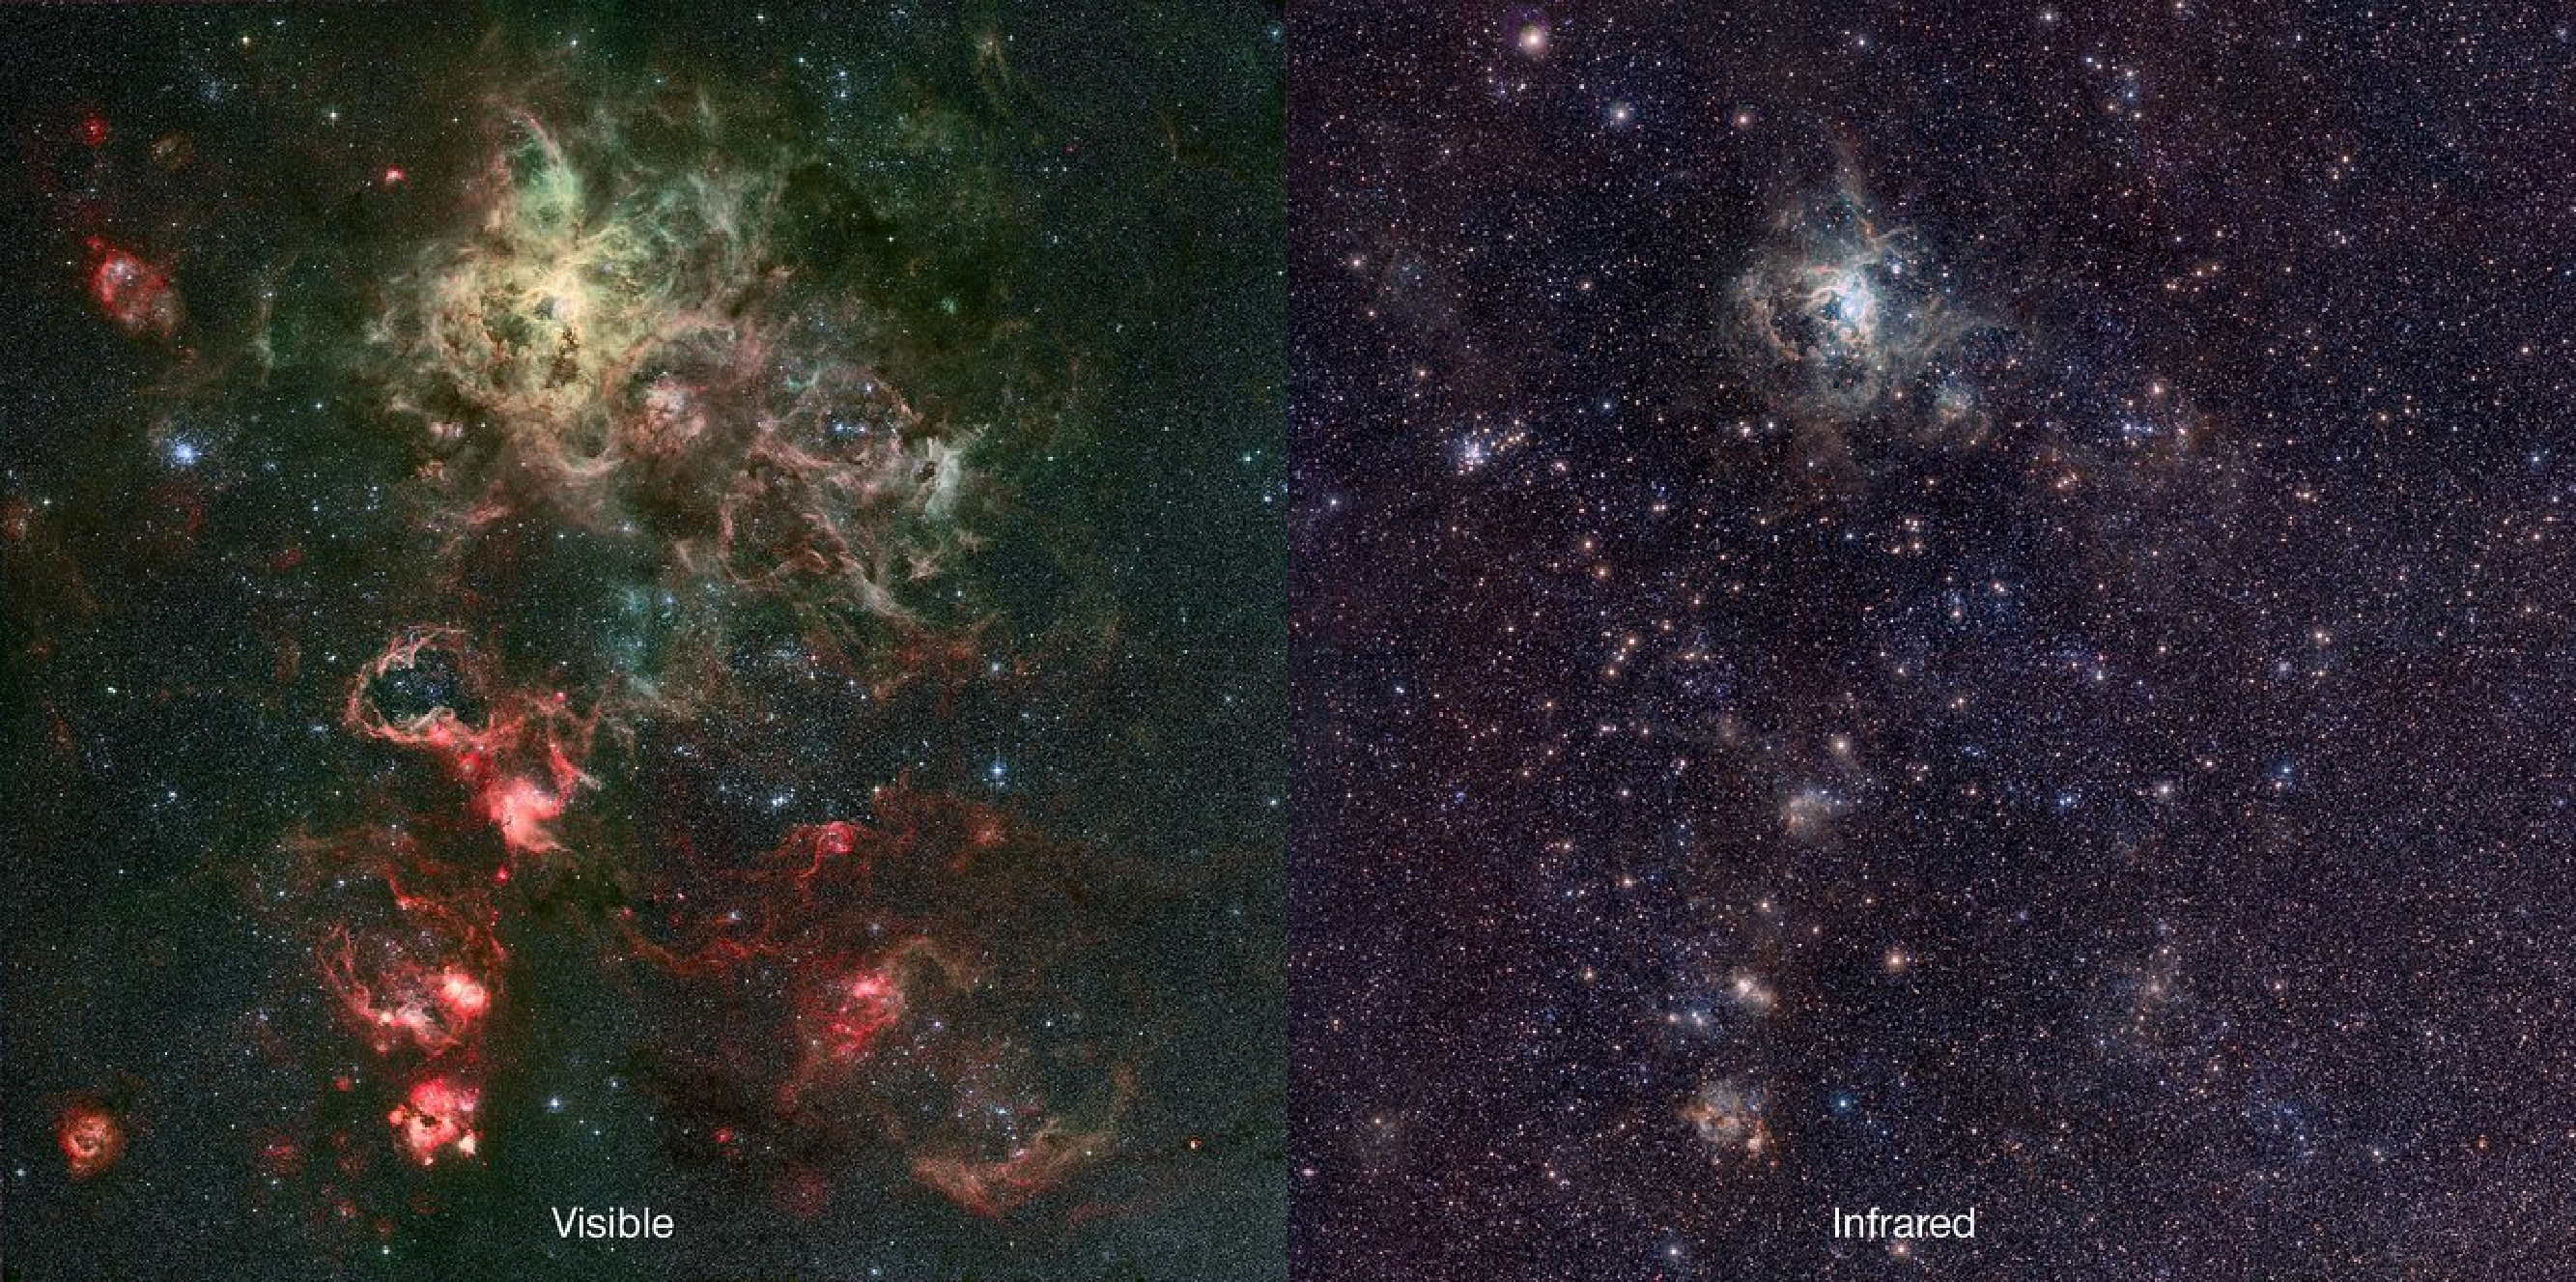
\includegraphics[height=3cm]{../illustrations/rgb_infrared}
    \hfill
    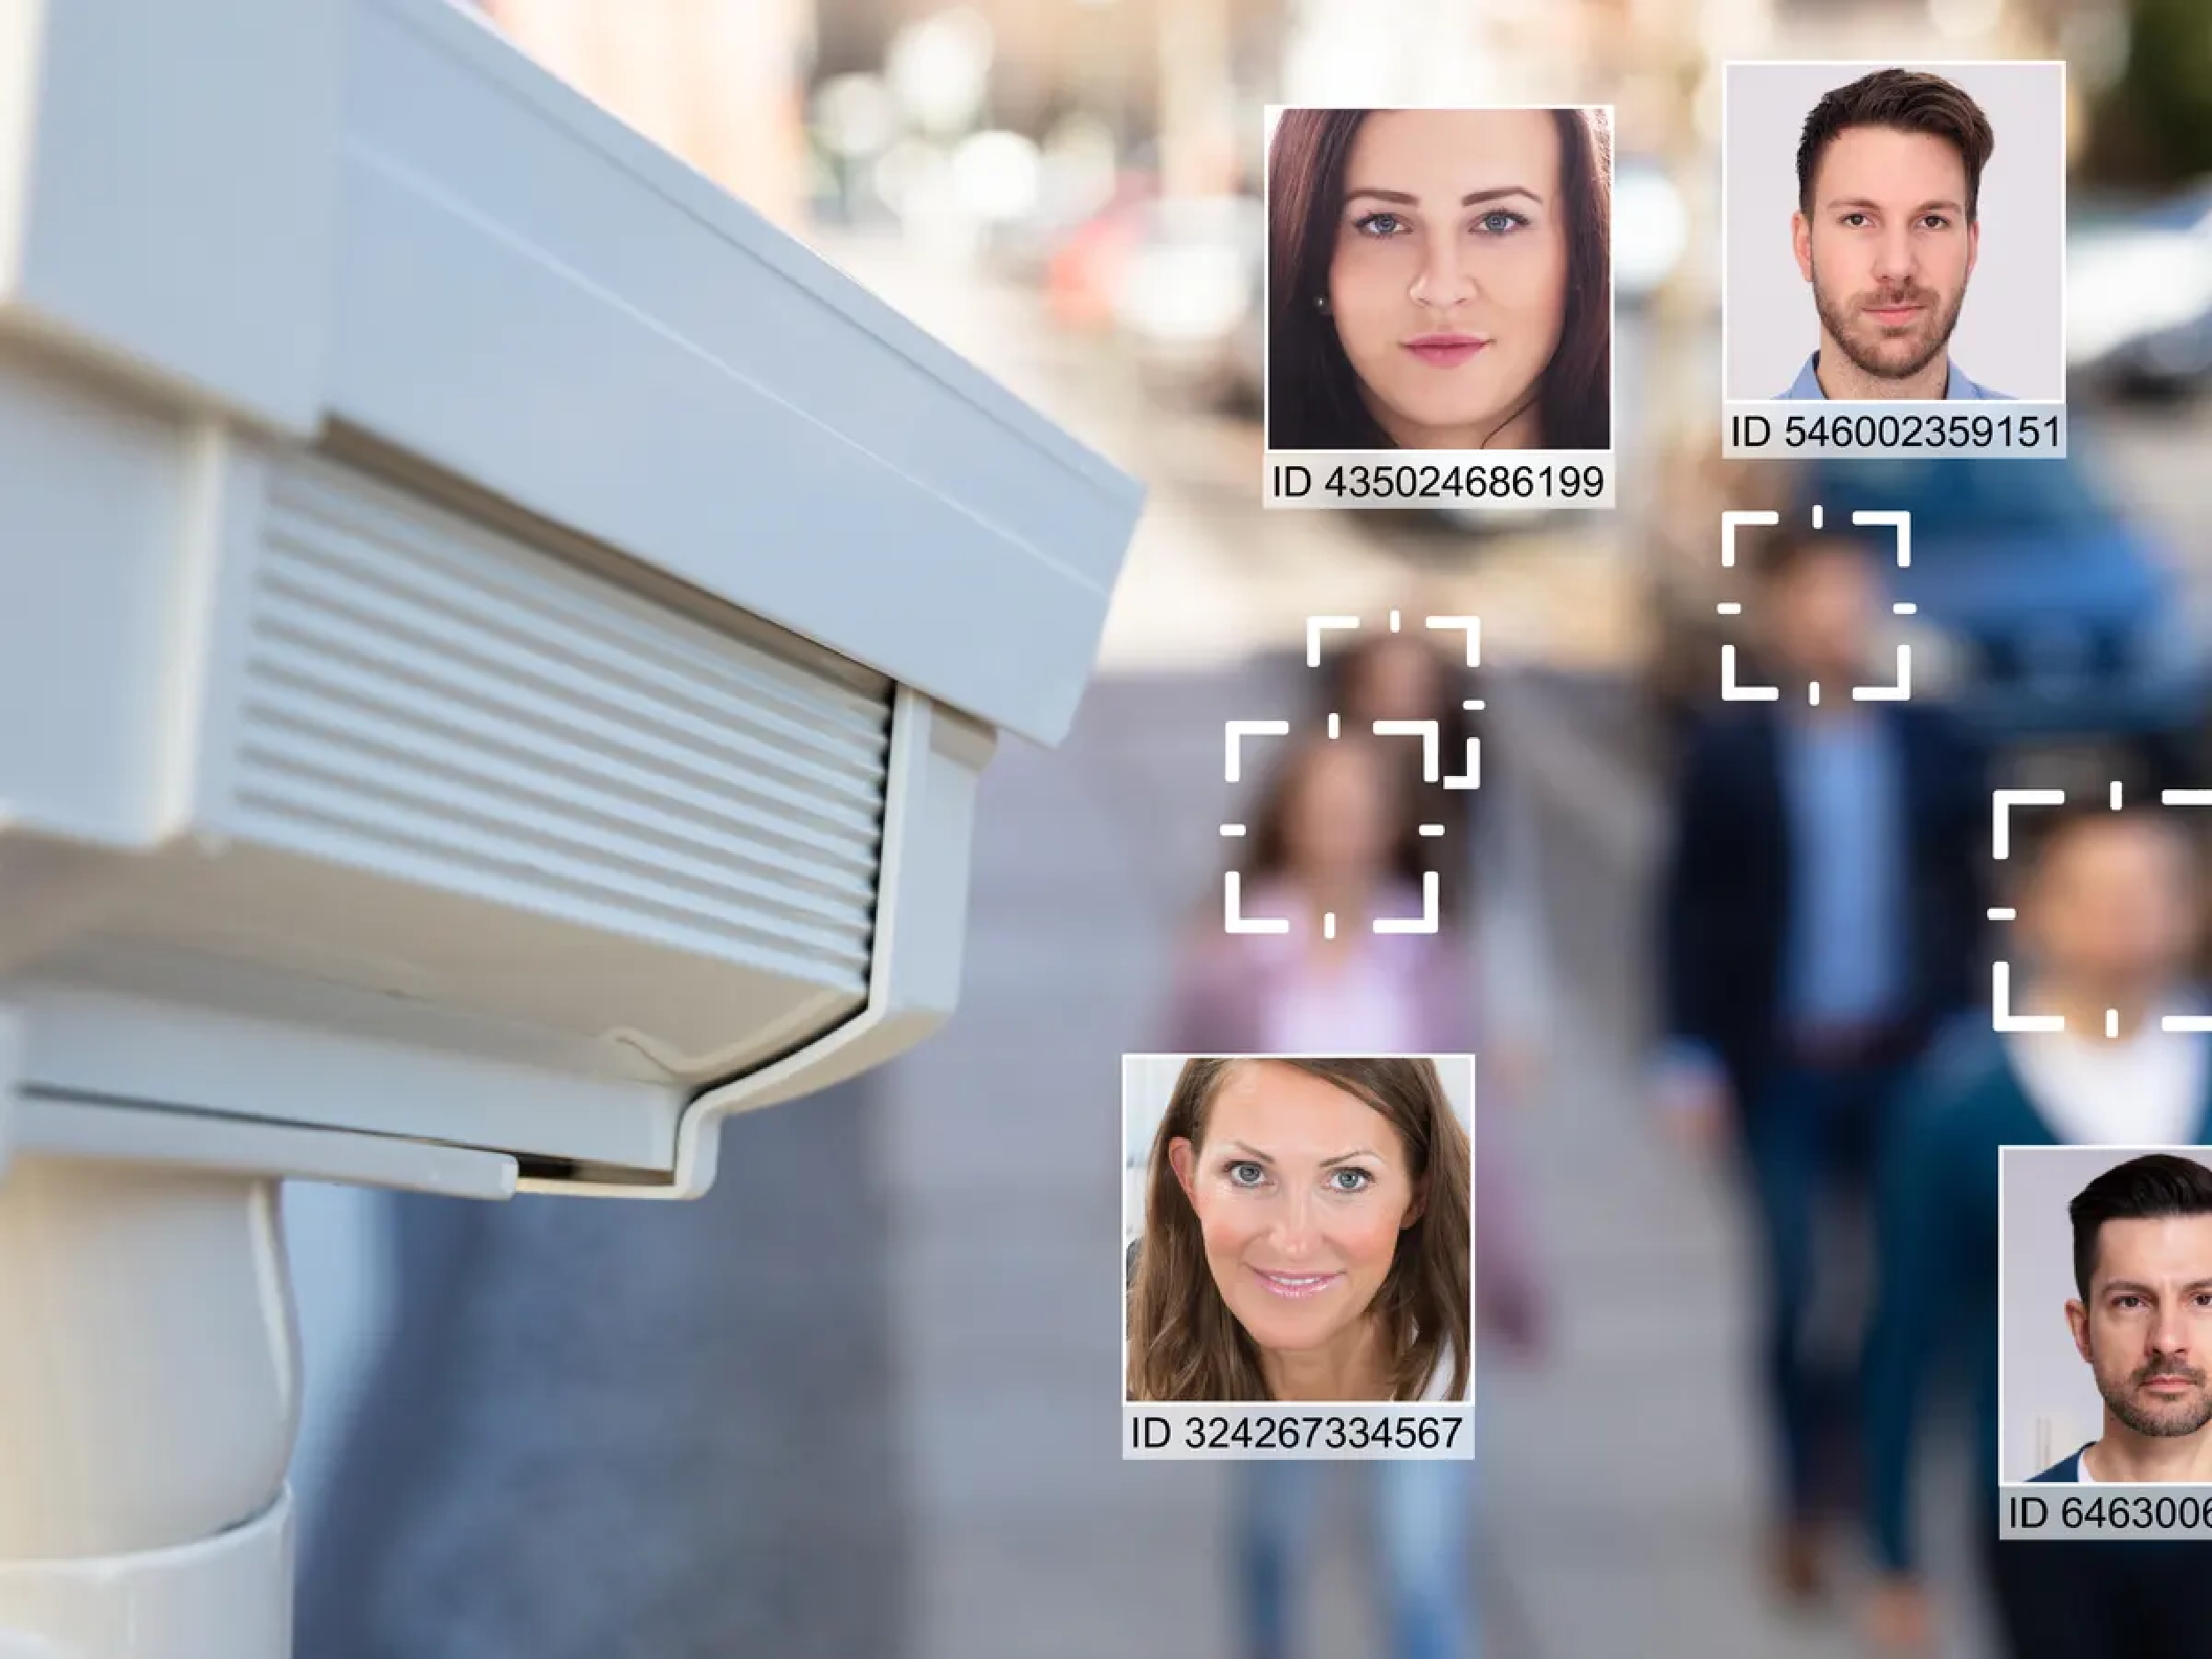
\includegraphics[height=3cm]{../illustrations/camera}
    \hspace{1cm}
  \end{figure}
\end{frame}

\begin{frame}[fragile]{Image processing nowadays}
  \begin{alertblock}{Different data types and algorithms}
    \begin{itemize}
      \item image-ND, hexagonal grid, cubical complexes value, etc.
      \item pixel-wise algorithms, local algorithms (convolution), global algorithms (propagation)
    \end{itemize}
  \end{alertblock}
  \begin{figure}[bl]
    \centering
    \hfill
    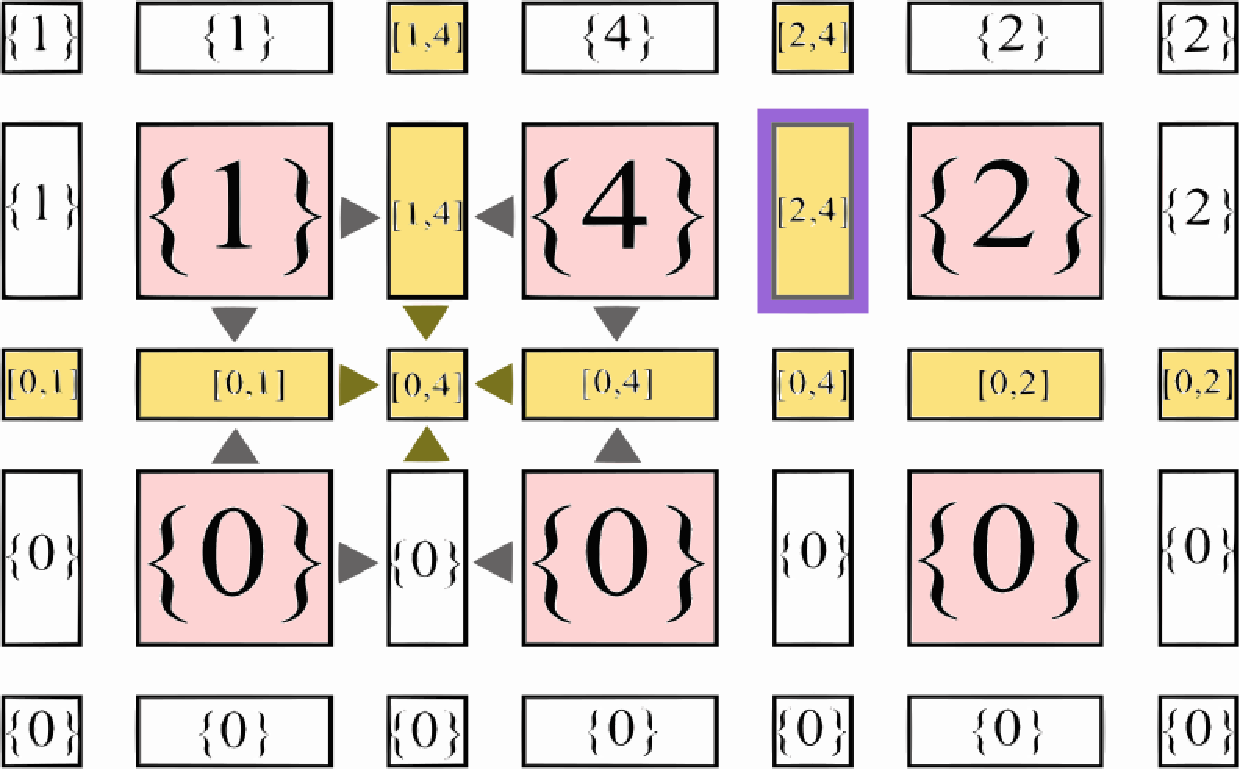
\includegraphics[height=2.3cm]{../illustrations/cubical_complex}
    \hfill
    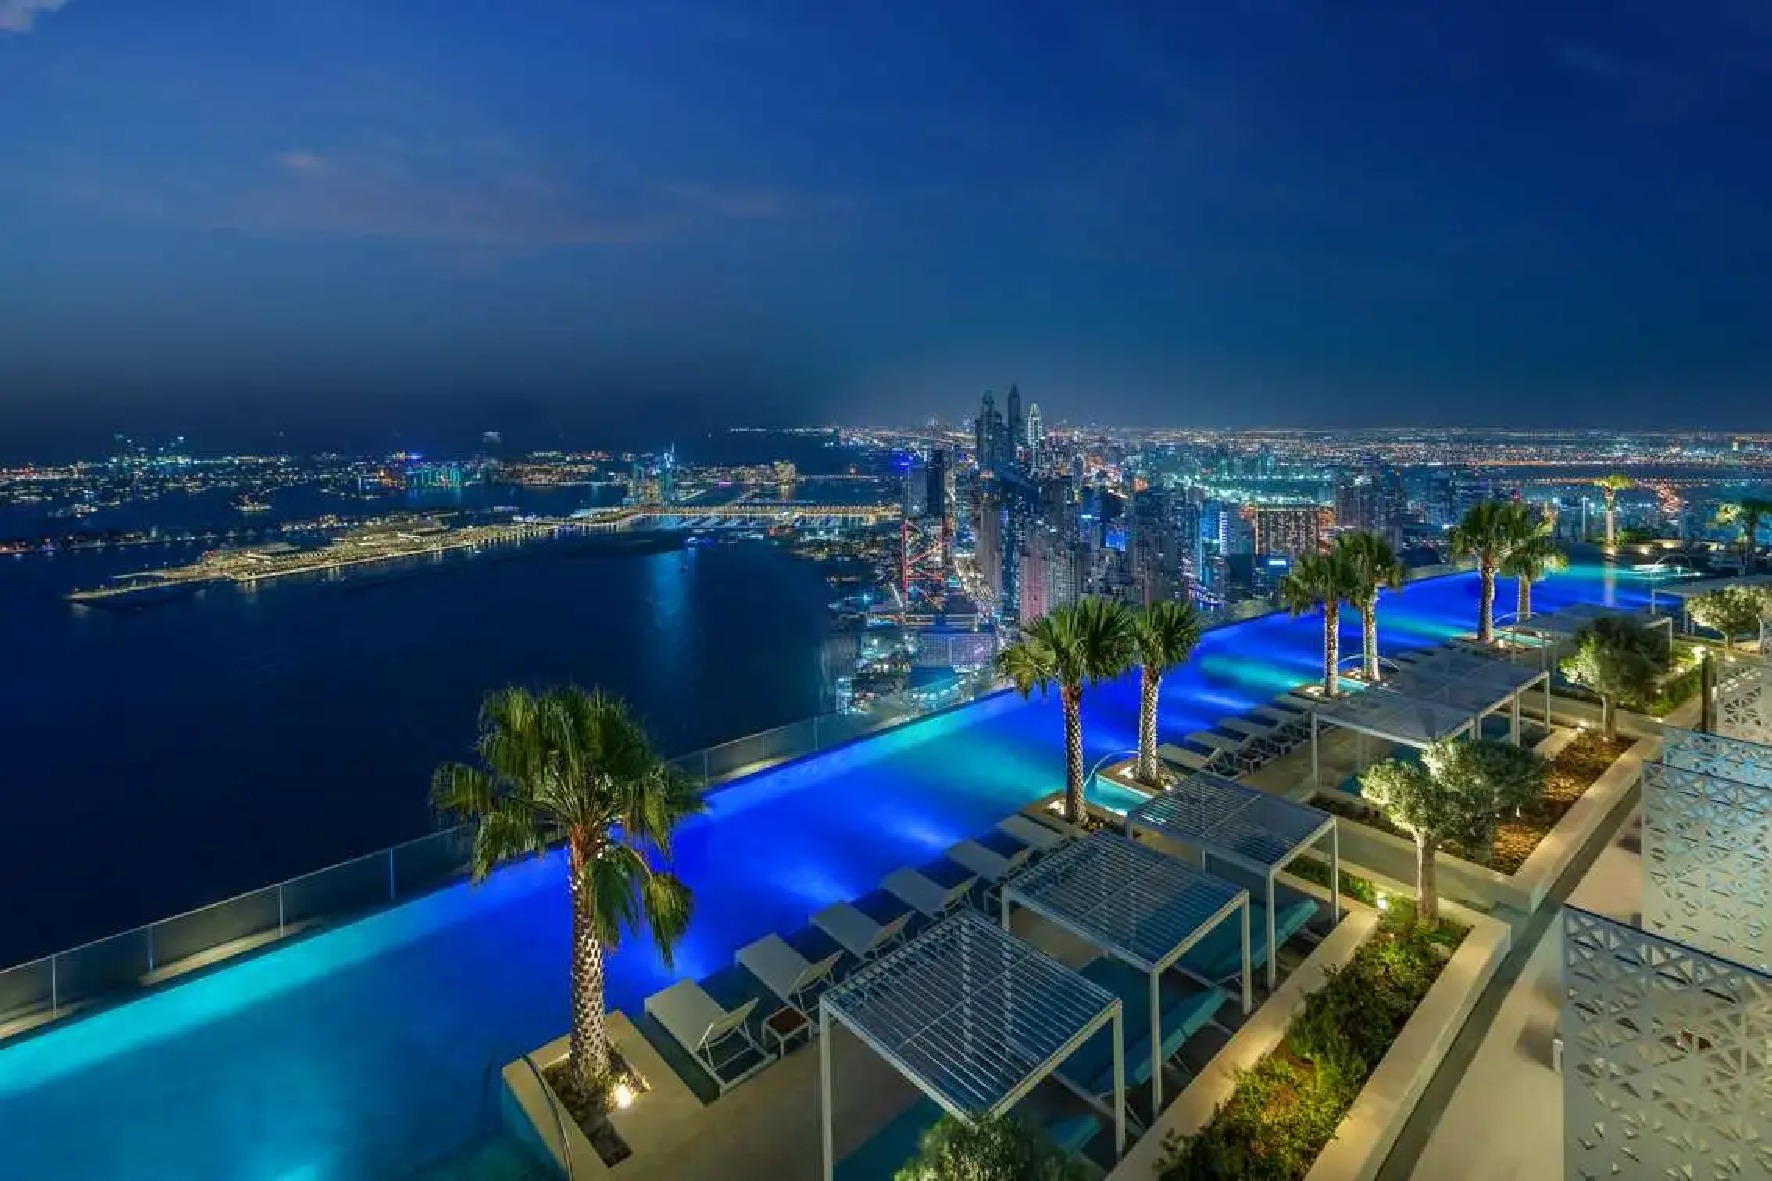
\includegraphics[height=2.3cm]{../illustrations/2d_rgb8_holiday_image}
    \hfill
    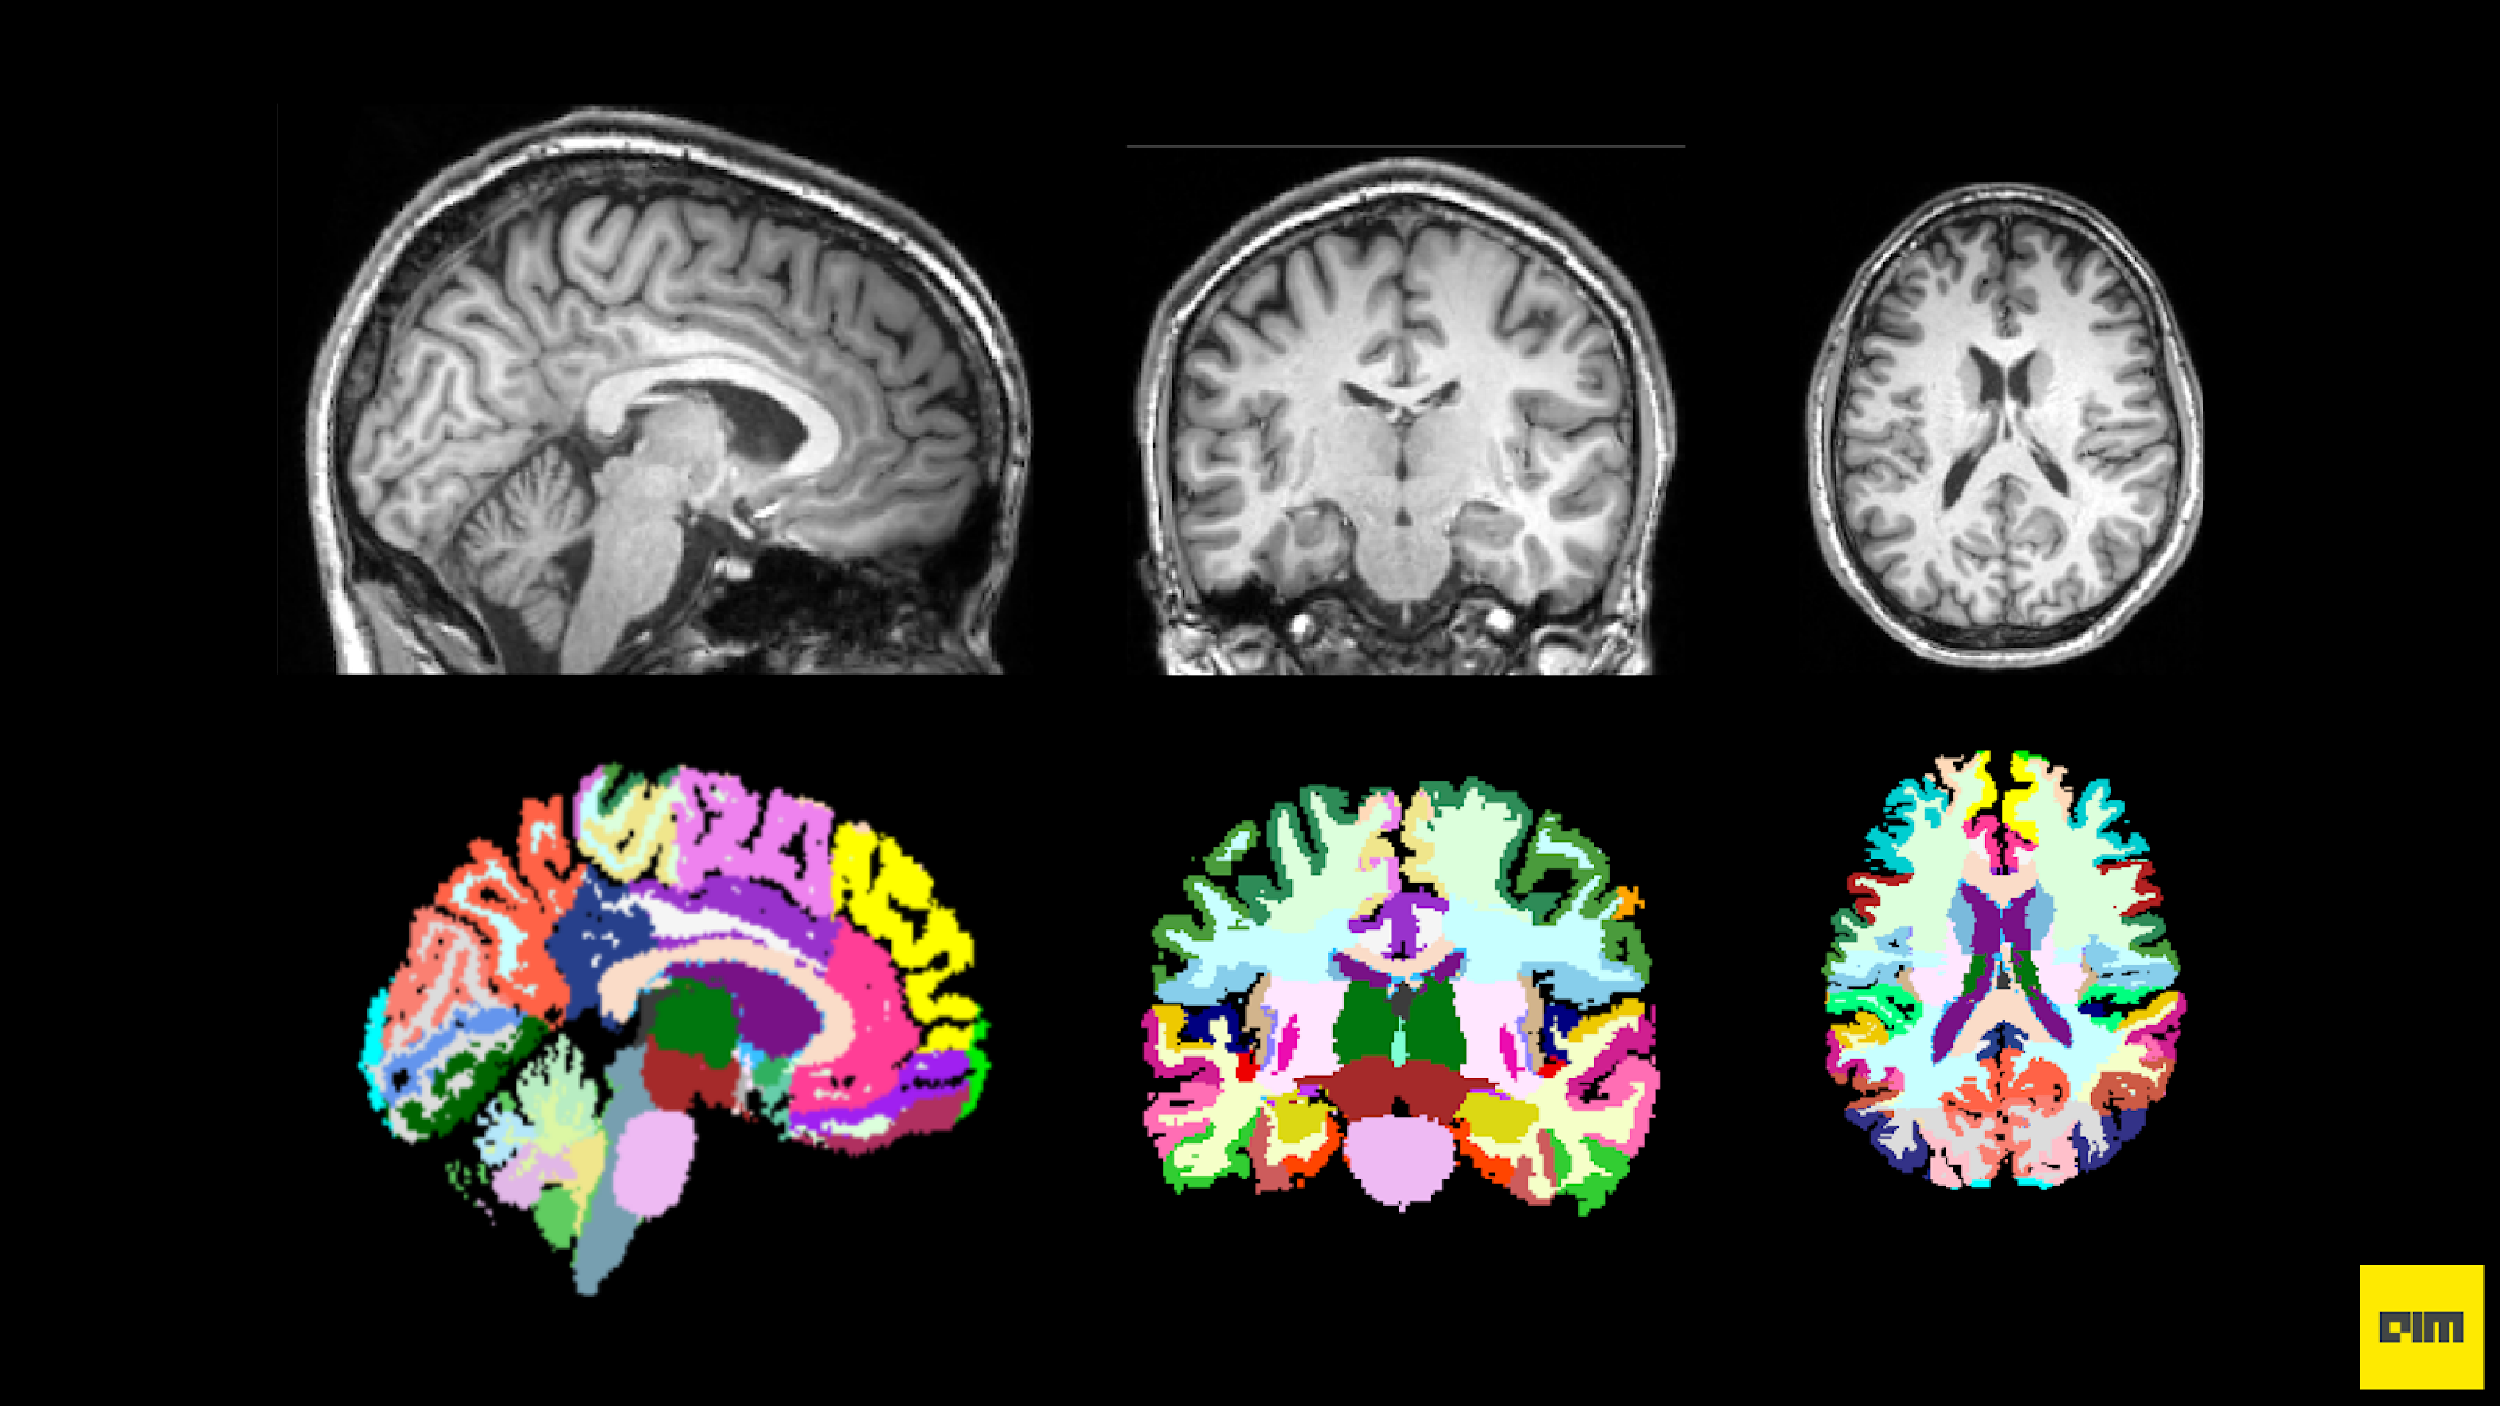
\includegraphics[height=2.3cm]{../illustrations/3d_medical_image}
    \hfill
    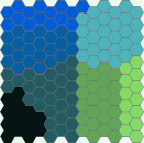
\includegraphics[height=2.3cm]{../illustrations/hexagonal_grid2}
    \hspace{1cm}
  \end{figure}
\end{frame}

\begin{frame}[fragile]{Image processing nowadays}
  \begin{alertblock}{Different user profiles and their use cases}
    \begin{itemize}
      \item The end user (non-programmer, wants UI interface).
      \item The practitioner (end user of an image processing library).
      \item The contributor (advanced user of a library familiar with its internals).
      \item The maintainer (founder/creator of the library or took it over to make it grow).
    \end{itemize}
  \end{alertblock}

  Our work is aimed toward the \emph{practitioner}, the \emph{contributor} and the \emph{maintainer}.
\end{frame}

\begin{frame}[fragile]{Image processing nowadays}
  \begin{alertblock}{Different tools}
    \begin{itemize}
      \item Graphic editors (GIMP, Photoshop).
      \item Command line utilities (ImageMagick, GraphicsMagick or MegaWave).
      \item Visual programming environment (Mathcad).
      \item Integrated environment (Matlab, Scilab, Octave, Mathematica and Jupyter).
      \item Package for Python (SciPy, NumPy, Scikit-image, Pillow or OpenCV bindings, via PyPi or Conda).
      \item \hl{Programming libraries (IPP, ITK, Boost.GIL, Vigra, Higra, GrAL, DGTal, OpenCV, CImg, Video++, Generic
              Graphic Library, Milena and Pylena.}
      \item Domain Specific Languages (DSL) (Eigen, Blaze, Blitz++ or Armadillo via C++ Expression template, or Halide
            and SYCL with their own toolchain).
    \end{itemize}
  \end{alertblock}
\end{frame}

\begin{frame}[fragile]{Need of Genericity for image processing}
  \begin{figure}[htbp]
    \raggedright\small
    \begin{tabular}{cccc}
                                                                              & image 2D
                                                                              & graph    & mesh \\[5pt]
      input:                                                                  &
      \fbox{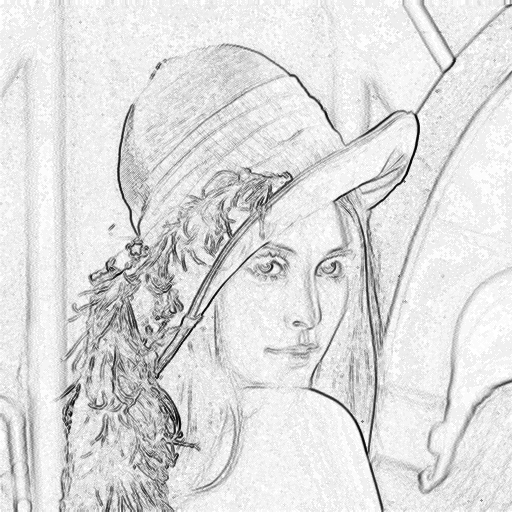
\includegraphics[width=.14\linewidth]{../figures/geninput-000b}}  &
      \fbox{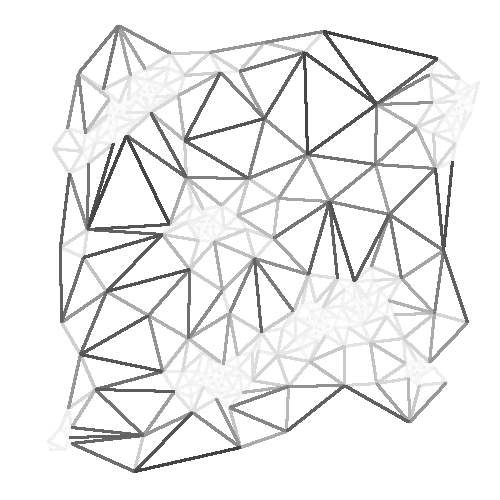
\includegraphics[width=.14\linewidth]{../figures/geninput-001b}}  &
      \fbox{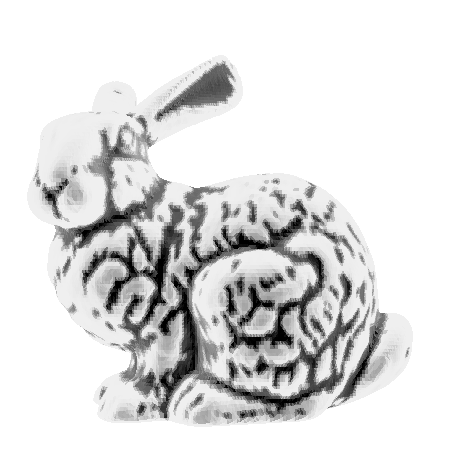
\includegraphics[width=.14\linewidth]{../figures/geninput-002b}}
      \\[5pt]
      %
      output:                                                                 &
      \fbox{
\includegraphics[width=.14\linewidth]{../figures/genoutput-000}}  &
      \fbox{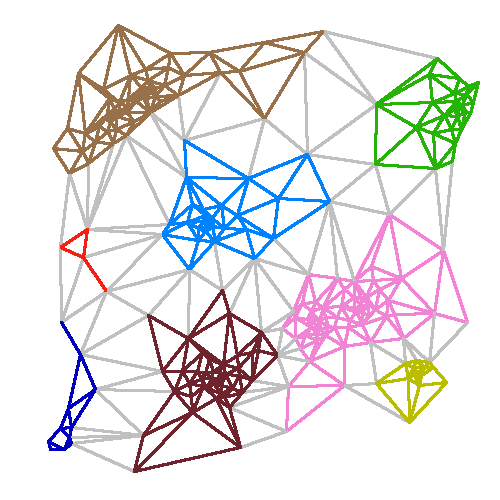
\includegraphics[width=.14\linewidth]{../figures/genoutput-001b}} &
      \fbox{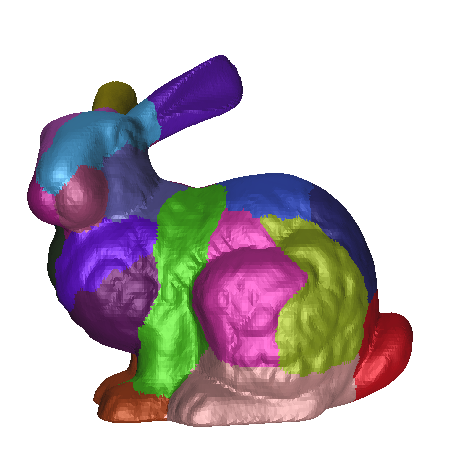
\includegraphics[width=.14\linewidth]{../figures/genoutput-002b}}
      \\
    \end{tabular}
    \label{fig:type.vs.algo}
    \caption{Watershed algorithm applied to three different image types.~\footfullcite{levillain.2014.ciarp}}
    %\vspace{-0.5cm}
    %\text{\textbf{Algorithms are intrinsically generics.}}
  \end{figure}
  \begin{textblock*}{4cm}(11cm,4cm)
    \textbf{Algorithms are intrinsically generic.}
  \end{textblock*}
\end{frame}

\begin{frame}[fragile]{Need of Genericity for image processing}
  Algorithm must support combination whose cardinality increases with:

  \begin{columns}[T,onlytextwidth]
    \column{0.48\textwidth}
    \begin{itemize}
      \item supported underlying image value type (grayscale, rgb, floating-point, \ldots)
      \item supported data structure (ND-buffers, graphs, meshes, \ldots)
      \item additional data type (structuring element, masks, \ldots)
    \end{itemize}

    \column{0.48\textwidth}
    \begin{figure}[htbp]
      \centering
      \includegraphics[width=0.8\textwidth]{../figures/possibility_space}
      \caption{Space of possibilities.}
      \label{fig:int.possibility_space}
    \end{figure}
  \end{columns}
\end{frame}

%
%
%

\AtBeginSection[]
{
  \begin{frame}{Outline}
    \setbeamertemplate{section in toc}[sections numbered]
    \vspace{0.2cm}
    \small%\singlespacing
    \tableofcontents[currentsection]
  \end{frame}
}

\section[Context and history of Generic Programming]{Context and history of Generic Programming}

\subsection[Unconstrained Genericity]{Unconstrained Genericity}

\begin{frame}[fragile]{Non-generic algorithm: gamma correction}
  Introducing the process of (generic) \textbf{Generalization}~\footfullcite{roynard.2019.rrpr}. \\
  Non-generic gamma-correction algorithm:
  \vspace{-0.3cm}
  \begin{minted}[linenos]{C++}
    void gamma_correction(Image& ima, double gamma)
    {
      const auto gamma_corr = 1.f / gamma;
      for (int x = 0; x < ima.width(); ++x)
        for (int y = 0; y < ima.height(); ++y)
        {
          ima(x, y).r = 256.f * std::pow(ima(x, y).r / 256.f, gamma_corr);
          ima(x, y).g = 256.f * std::pow(ima(x, y).g / 256.f, gamma_corr);
          ima(x, y).b = 256.f * std::pow(ima(x, y).b / 256.f, gamma_corr);
        }
    }
  \end{minted}
  \begin{textblock*}{4cm}(11cm,1.5cm)
    This algorithm is \textbf{over-constrained}. \\
    How can we make it \textbf{Generic}?
  \end{textblock*}
\end{frame}

\begin{frame}[fragile]{1rst approach: Code duplication}
  \begin{itemize}
    \item Writing and optimizing an algorithm for a particular data type in mind.
    \item Often results in multiple switch/cases to enumerate all the supported combination of supported data types.
  \end{itemize}
  \begin{minted}{C++}
    void gamma_correction(any_image img, double gamma)
    {
      switch((img.structure_kind, img.value_kind)) 
      {
      case (BUFFER2D, UINT8):
        gamma_correction_img2d_uint8( (image2d<uint8>) img, gamma );
      // ...
      case (LUT, RGB8):
        gamma_correction_lut_rgb8( (image_lut<rgb8>) img, gamma );
      // ...
      }
    }
  \end{minted}
\end{frame}

\begin{frame}[fragile]{2nd approach: Generalization}
  \begin{itemize}
    \item Necessity to have a common denominator to all the supported types: the super-type.
    \item All supported data types must be convertible to and from this super-type.
    \item Good for maintenance but conversions impact performance.
  \end{itemize}
  \begin{minted}{C++}
    struct image4D { // generalized super-type with generalized underlying value-type
      using value_type = std::array<double, 4>; // every value is converted to this one
    }; // specific types w/ conversion routines
    struct image2D { image4D to(); void from(image4D); };
    struct image3D { image4D to(); void from(image4D); };
    void gamma_correction(image4D img, double gamma) {
      for(auto row : img.rows())
        for(auto z_row : row.rows())
          for(auto y_row : z_row.rows())
            for(auto x : y_row.pixels())
              auto& v = x.val(); // image4D::value_type
              // correct v with gamma
    }
  \end{minted}
\end{frame}

\begin{frame}[fragile]{3rd approach: Inclusion Polymorphism}
  \begin{itemize}
    \item Extracting behavior pattern from algorithms
    \item Grouping them into logical bricks called \textbf{interfaces}.
    \item Each algorithm can require a set of behavioral pattern to be satisfied.
    \item \hl{All happens at runtime} (dynamic dispatch).
  \end{itemize}

  \begin{columns}[T,onlytextwidth]
    \column{0.48\textwidth}
    \centering
    \includegraphics[width=0.8\textwidth]{../figures/inclupoly}

    \column{0.48\textwidth}
    \centering
    \includegraphics[width=0.8\textwidth]{../figures/inclupoly_code_gamma}
  \end{columns}
\end{frame}

\begin{frame}[fragile]{4th approach: Parametric Polymorphism}
  \begin{itemize}
    \item Extracting behavior pattern from algorithms
    \item Grouping them into logical bricks called \textbf{concepts}.
    \item Each algorithm can require a set of behavioral pattern to be satisfied.
    \item \hl{All happens at compile-time} (static dispatch).
  \end{itemize}

  \begin{columns}[T,onlytextwidth]
    \column{0.48\textwidth}
    \centering
    \includegraphics[width=0.65\textwidth]{../figures/parapoly}

    \column{0.48\textwidth}
    \centering
    \includegraphics[width=0.8\textwidth]{../figures/parapoly_code_gamma}
  \end{columns}
\end{frame}

\begin{frame}[fragile]{Genericity within Libraries}
  All existing library do not fall into one single category and combine those techniques to achieve diverse degree of
  genericity.
  \vspace{-0.2cm}\small\begin{itemize}
    \item CImg mixes \emph{Generalization} and \emph{Parametric polymorphism} by considering only 4D-images parametrized
          by their value type.
    \item OpenCV's algorithms take polymorphic input types (Inclusion polymorphism) but dispatch on the value type on
          specialized algorithm (code duplication) that then re-dispatch on generic routines (parametric polymorphism).
    \item Scikit-image relies on Scipy which uses dynamic abstraction (inclusion polymorphism) for its nd-array and
          sometimes dispatch on specialized routine (code duplication) for performance.
    \item Many other libraries have chosen to leverage Parametric polymorphism at diverse degree (Boost.GIL, Higra,
          Vigra, GrAL, DGTal, Milena and Pylene)
  \end{itemize}
\end{frame}

\begin{frame}[fragile]{Genericity: Summary}
  \begin{table}[htbp]
    \centering
    \small
    \begin{threeparttable}
      %\caption{Genericity approaches: pros.~\&~cons.}
      \begin{tabular}[width=0.8\linewidth]{l|ccccc}
        Paradigm             & TC\tnote{1} & CS\tnote{2} & E\tnote{3} & One IA\tnote{4} & EA\tnote{5} \\
        \hline
        Code Duplication     & \cmark      & \xmark      & \cmark     & \xmark          & \xmark      \\
        Code Generalization  & \xmark      & \eqmark     & \eqmark    & \cmark          & \xmark      \\
        Object-Orientation   & \eqmark     & \cmark      & \xmark     & \cmark          & \cmark      \\
        Generic Programming: &             &             &            &                 &             \\
        \quad with C++11     & \cmark      & \eqmark     & \cmark     & \cmark          & \eqmark     \\
        \quad with C++17     & \cmark      & \cmark      & \cmark     & \cmark          & \eqmark     \\
        \quad with C++20     & \cmark      & \cmark      & \cmark     & \cmark          & \cmark      \\
      \end{tabular}
      \begin{tablenotes}
        \item[1] TC: type checking.
        \item[2] CS: code simplicity.
        \item[3] E: efficiency.
        \item[4] One IA: one implementation per algorithm.
        \item[4] EA: explicit abstractions / constrained genericity.
      \end{tablenotes}
      \label{table:gen.approaches}
    \end{threeparttable}
  \end{table}
\end{frame}

\subsection[Toward constrained Genericity]{Toward constrained Genericity}

\begin{frame}[fragile]{Toward constrained genericity: Step 1}
  Lifting RGB constraint:
  \begin{minted}[linenos,highlightlines={3,6,10},highlightcolor=yellow!60!white]{C++}
    void gamma_correction(Image& ima, double gamma)
    {
      using value_t = typename Image::value_type;

      const auto gamma_corr = 1.f / gamma;
      const auto max_val = std::numeric_limits<value_t>::max();
    
      for(int x = 0; x < ima.width(); ++x)
        for(int y = 0; y < ima.height(); ++y)
          ima(x, y) = max_val * std::pow(ima(x, y) / max_val, gamma_corr);
    }
  \end{minted}
  \begin{textblock*}{4cm}(11.5cm,3cm)
    \textbf{There is no valid reason to constrain this algorithm to RGB images.}
  \end{textblock*}
\end{frame}

\begin{frame}[fragile]{Toward constrained genericity: Step 2}
  Lifting 2-dimensional constraint:
  \begin{minted}[linenos,highlightlines={8-9},highlightcolor=yellow!60!white]{C++}
    void gamma_correction(Image& ima, double gamma)
    {
      using value_t = typename Image::value_type;

      const auto gamma_corr = 1.f / gamma;
      const auto max_val = std::numeric_limits<value_t>::max();
    
      for (auto&& pix : ima.pixels())
        pix.val() = max_val * std::pow(pix.value() / max_val, gamma_corr);
    }
  \end{minted}
  \begin{textblock*}{4cm}(11.5cm,3cm)
    \textbf{There is no valid reason to constrain this algorithm to 2D-images.}
  \end{textblock*}
\end{frame}

\begin{frame}[fragile]{Toward constrained genericity: Constraints so far}
  \begin{alertblock}{Prerequisite for the algorithm}
    \begin{itemize}
      \item \texttt{Image} type provides subtype \texttt{value\_type}.
      \item \texttt{Image} type provides a member function \texttt{pixels()} for traversing.
      \item Underlying image's value type has a maximum bound.
      \item Underlying image's value type behaves properly with \texttt{pow}.
    \end{itemize}
  \end{alertblock}
  \textbf{Issue: Genericity is unconstrained, so the check is done late and error messages are infamously complicated.}
\end{frame}

\begin{frame}[fragile]{Old techniques (pre-C++20)}
  Before C++20 (2020) we relied on metaprogramming techniques to achieve constrained Genericity:
  \vspace{-0.2cm}\begin{itemize}
    \item Functions on types: metafunctions or type-traits
    \item SFINAE: Substitution Failure Is Not An Error
    \item CRTP: Curiously Recurring Template Pattern (used in the SCOOP paradigm~\footfullcite{geraud.2008.mpool} in Milena).
  \end{itemize}
  \vspace{-0.3cm}
  \begin{center}\textbf{We do not want this anymore!}\end{center}
\end{frame}

\begin{frame}[fragile]{Final step: Conceptification 1/2}
  C++ introduce the syntax for Concepts:
  \begin{columns}[T,onlytextwidth]
    \column{0.50\textwidth}
    \begin{minted}{C++}
template <class I>
concept Image = requires {
    typename I::value_type; // type of value
    typename I::point_type; // type of points
    typename I::pixel_type; // type of pixels
  } &&
  Pixel<I::pixel_type> &&
  requires (I ima) {
    { ima.pixels() } -> mdrange<I::pixel_type>;
  };
template <Image I>
concept WritableImage = 
  WritablePixel<I::pixel_type> &&
  requires (I ima) {
    { ima.pixels() } -> mdrange<I::pixel_type>;
  };
  \end{minted}

    \column{0.50\textwidth}
    \begin{minted}{C++}
    template <class P>
    concept Pixel = requires {
        typename I::value_type; // type of value
        typename I::point_type; // type of points
      } && requires (P pix) {
        { pix.val() } -> I::value_type;
        { pix.pnt() } -> I::point_type;
      };
    template <Pixel P>
    concept WritablePixel = 
      requires (P pix, P::value_type v) {
        { pix.val() = v };
      };
  \end{minted}
  \end{columns}
\end{frame}

\begin{frame}[fragile]{Final step: Conceptification 2/2}
  \begin{minted}[linenos,highlightlines={1-4},highlightcolor=yellow!60!white,escapeinside=||]{C++}
    template <|\colorbox{red}{WritableImage}| Image>
      requires requires(Image::value_type v, double d) {
        { std::pow(v, d) } -> Image::value_type;
      }
    void gamma_correction(Image& ima, double gamma)
    {
      using value_t = typename Image::value_type;
    
      const auto gamma_corr = 1.f / gamma;
      const auto max_val = std::numeric_limits<value_t>::max();
    
      for (auto&& pix : ima.pixels())
        pix.val() = max_val * std::pow(pix.value() / max_val, gamma_corr);
    }
  \end{minted}
  \vfill
  \begin{center}\textbf{This is the final (most generalized) version of the algorithm.}\end{center}
  \begin{textblock*}{4cm}(11.5cm,3.2cm)
    \textbf{A \emph{Concept} is a set of behavioral requirement (constraints) applied to a type.}
  \end{textblock*}
\end{frame}

%
%
%
\section[Generic Programming for Image Processing in the static world (contribution)]{Generic programming for Image Processing in the static world (contribution)}

\subsection{Taxonomy of Image Processing algorithms}

\begin{frame}{Taxonomy for Image Processing: Goal}
  \begin{alertblock}{Taxonomy definition}
    Act of doing a classification of something in a systematic way.
  \end{alertblock}
  \begin{itemize}
    \item Provide zero-costs abstractions so that algorithm families can work on image type families.
    \item Code will be easy and efficient by default.
  \end{itemize}
  \begin{center}
    \textbf{Concepts are not designed after data structures but after algorithms.}
  \end{center}
\end{frame}

\begin{frame}[fragile]{Taxonomy of Image Processing algorithms: three families}
  \begin{itemize}
    \item Pixel-wise algorithms: thresholding, gamma correction.
    \item Local algorithms: dilation, erosion, closing, hit-or-miss, gradient, rank filter, etc.
    \item Global algorithms: Chamfer distance transform, labeling, union-find, max-tree, etc.
  \end{itemize}
  From those families emerge several concepts.
\end{frame}

\subsection{Concepts for Image Processing algorithms}

\begin{frame}[fragile]{Our Concepts for Image Processing: fundamentals}
  Fundamental concepts are necessary to be able to do basic manipulations over an image.
  \begin{itemize}
    \item Value, Point, Pixels: represent the trivial building blocks of an image.
    \item Domain: represent the set of points valid for a given image (definition domain).
    \item Image: represent the algebraic relation \(y = f(x)\) where \(y\) is a value generated by the image \(f\) for
          the input (point) \(x\).
    \item Aside from generating a value, an image can also store a value, as in \(f(x) = y\).
  \end{itemize}
  Concepts interact with each other's through \hl{composition} and \hl{refinement} (close to inheritance).
\end{frame}

\begin{frame}[fragile]{Our Concepts for Image Processing: fundamentals}
  The basic use case of an image is illustrated by the following code:
  \begin{minted}{C++}
    auto ima = Image();           // Get an image
    for(auto pix : ima.pixels()) {  // Traverse the image
      auto pnt = pix.point();       // Get the pixel's point
      auto& val = pix.value();      // Get the pixel's value
      val = 42;                     // Set the pixel's value
    }
  \end{minted}
\end{frame}

\begin{frame}[fragile]{Our Concepts for Image Processing: Image concept}
  \centering
  \begin{figure}
    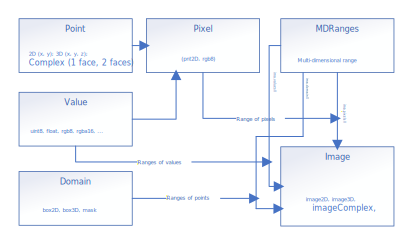
\includegraphics[width=0.9\textwidth]{../figures/concepts/image}
  \end{figure}
\end{frame}

\begin{frame}[fragile]{Our Concepts for Image Processing: Pixel concept}
  \centering
  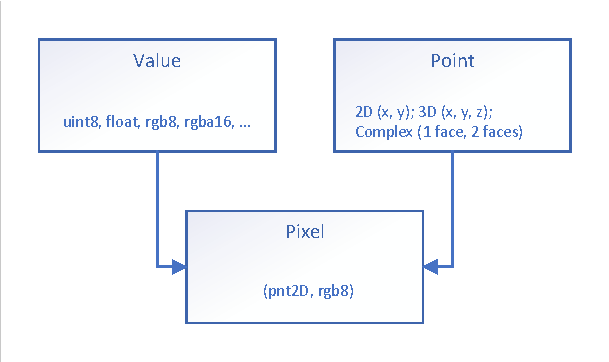
\includegraphics[width=0.5\textwidth]{../figures/concepts/pixel}
  \begin{minted}{C++}
  auto pix = Pixel();     // Get a pixel
  auto val = pix.val();   // yield the pixel value
  auto pnt = pix.point(); // yield the pixel point
  pix.val() = 42;         // Assign a value
  \end{minted}
\end{frame}

\begin{frame}[fragile]{Our Concepts for Image Processing: Domain concept}
  \centering
  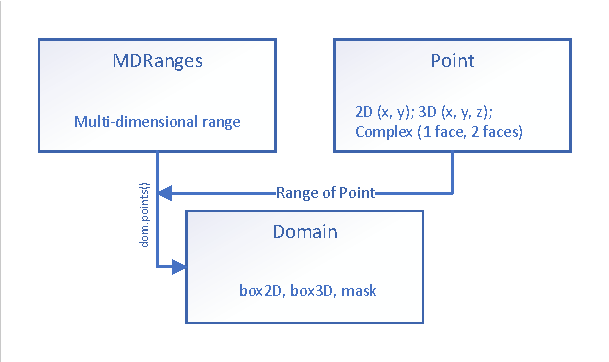
\includegraphics[width=0.45\textwidth]{../figures/concepts/domain}
  \begin{minted}{C++}
    auto dom = Domain();          // Get a domain
    auto pnt = Point(..., ...);   // Get a random point
    bool ret = dom.has(pnt);      // Check wether the domain contains the point
    bool is_empty = dom.empty();  // Check wether the domain is empty
    auto dim = dom.dim();         // Yield the domain's dimension information
    for(auto pnt : dom)           // browse the definition domain
      // use pnt as a point of the domain
  \end{minted}
\end{frame}

\begin{frame}[fragile]{Our Concepts for Image Processing: Advanced Image concept}
  \begin{itemize}
    \item IndexableImage: traversing an image via indexes.
          \begin{minted}{C++}
      auto v = ima[k]; // Access value from an index
    \end{minted}
    \item AccessibleImage: accessing image's value through points.
          \begin{minted}{C++}
      auto v = ima(pnt);   // Access value from a point
    \end{minted}
    \item BidirectionalImage: traversing image forward and backward for global algorithm such as Chamfer distance
          transform that needs a forward pass and a backward pass.
          \begin{minted}{C++}
      for(auto pix : ima.pixels()) // forward pass
      for(auto pix : reversed(ima.pixels())) // backward pass
    \end{minted}
    \item RawImage: direct access to the image's data buffer.
          \begin{minted}{C++}
      const int* data = ima.data(); // Access the underlying buffer
      auto dim = ima.domain().dim(); // Get the dimension of the image
      // Retrieve information about strides
      auto strides = std::vector<std::ptrdiff_t>(0, dim)
      for (int i = 0; i < dim; ++i)
        strides[i] = ima.stride(i)
      \end{minted}
  \end{itemize}
\end{frame}

\begin{frame}[fragile]{Our Concepts for Image Processing: Advanced Image concept}
  \centering
  \begin{figure}
    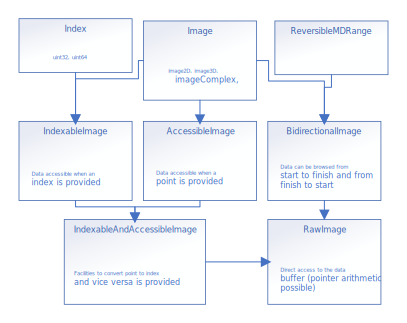
\includegraphics[width=0.65\textwidth]{../figures/concepts/images_all}
  \end{figure}
\end{frame}


\begin{frame}[fragile]{Our Concepts for Image Processing: Local algorithms}
  \begin{itemize}
    \item Support for structuring elements (disc, rectangle, sphere, cube, etc.)
    \item Support for extension (flat buffer, unique value, mirroring, etc.)
  \end{itemize}
  Typical usage in local algorithms:

  \begin{minted}{C++}
      auto se = se::disc(.radius=3); // get a structuring element
      for(auto pix : ima.pixels())   // traverse image
        for(auto nbx : se(pix))       // traverse neighboring pixels
          // nbx is a range of pixels
  \end{minted}
\end{frame}

\begin{frame}[fragile]{Our Concepts for Image Processing: Local algorithms}
  \centering
  \begin{figure}
    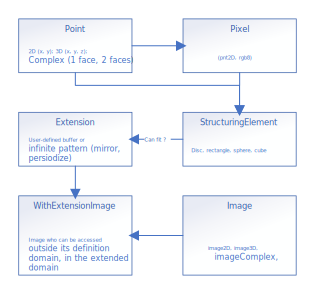
\includegraphics[width=0.7\textwidth]{../figures/concepts/se_extension}
  \end{figure}
\end{frame}

\subsection{Algorithms canvas}

\begin{frame}[fragile]{0-overhead for designed abstraction}
  \begin{itemize}
    \item We designed abstraction around those concepts that enables 0-overhead when they are used properly.
    \item For the majority of cases the default code will be the most efficient.
    \item It is possible to dispatch (dynamically of statically) to algorithms specialization for the remaining edge
          cases for maximum efficiency.
  \end{itemize}
  \begin{columns}[T,onlytextwidth]
    \column{0.50\textwidth}
    \begin{minted}{C++}
template <Image Img, StructuringElement SE>
auto dilate(Img img, SE se) {
  if (se.is_decomposable()) {
    lst_small_se = se.decompose();
    for (auto small_se : lst_small_se)
      // Recursive call
      img = dilate(img, small_se);
    return img;
  }
    \end{minted}

    \column{0.50\textwidth}
    \begin{minted}{C++}
  else if (is_pediodic_line(se))
      // Van Herk's algorithm
    return fast_dilate1d(img, se);
  else
      // Classic algorithm
    return dilate_normal(img, se);
}
    \end{minted}

    %\column{0.40\textwidth}
    %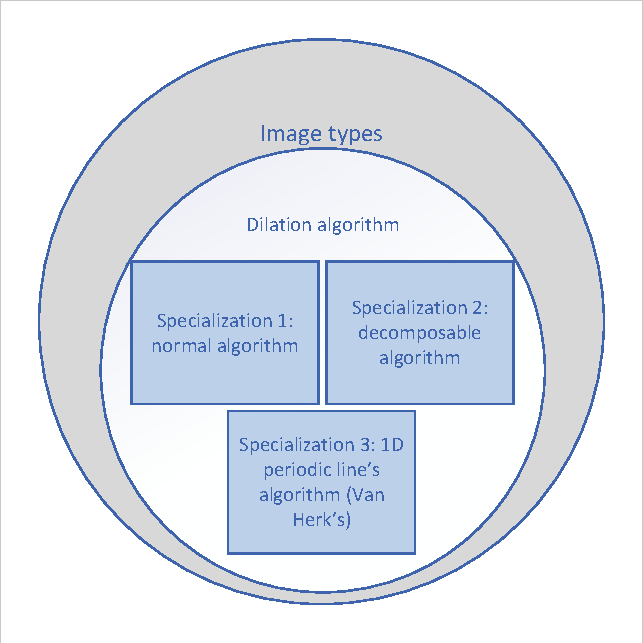
\includegraphics[width=0.99\textwidth]{../figures/dilation_specialization_diagram}
  \end{columns}
\end{frame}

\begin{frame}[fragile]{Taxonomy for Image Processing: Canvas for Dilation \& Erosion}
  Dilation and Erosion have the same shape:
  \begin{columns}[T,onlytextwidth]
    \column{0.50\textwidth}
    \includegraphics[width=0.7\textwidth]{../figures/dilation_code}

    \column{0.50\textwidth}
    \includegraphics[width=0.7\textwidth]{../figures/erosion_code}
  \end{columns}
  \bigskip
  They can be rewritten in a common canvas:
  \begin{columns}[T,onlytextwidth]
    \column{0.50\textwidth}
    \includegraphics[width=1.1\textwidth]{../figures/local_op_code}

    \column{0.50\textwidth}
    \includegraphics[width=0.6\textwidth]{../figures/local_op_dilation_code}
    \includegraphics[width=0.6\textwidth]{../figures/local_op_erosion_code}
  \end{columns}
\end{frame}

\begin{frame}[fragile]{Taxonomy for Image Processing: Algorithms over-generalization}
  \begin{itemize}
    \item Algorithms can have the same computational shape.
    \item When this shape is known, an algorithm canvas can be written (meta-algorithm)
    \item This canvas shifts the algorithm implementation into a descriptive paradigm.
    \item This canvas allows reusing code easily.
    \item This canvas allows the maintainer to factorize optimizations (GPU offloading, etc.)
  \end{itemize}
\end{frame}

%
%
%
\section[Views for Image Processing (contribution)]{Views for Image Processing (contribution)}

\subsection{Genesis of a new abstraction layer: Views}

\begin{frame}[fragile]{Views for Image Processing}
  \begin{alertblock}{View definition}
    A view is an \emph{image} which embarks an algorithm and features properties. They are inspired from Milena's
    morphers~\footfullcite{levillain.2009.ismm} and STL ranges~\footfullcite{niebler.2014.ranges}. We published our take
    in~\footfullcite{roynard.2022.gpce}.

    In Pylene, \hl{a View \textbf{IS} an Image} and \hl{all Image are lightweight} objects (cheap-to-copy). Images have
    \hl{value semantic} and copies perform \emph{shallow-copies} with a shared data buffer by default.
  \end{alertblock}
  \begin{center}\textbf{Views can replace pixel-wise algorithms.}\end{center}
\end{frame}

\begin{frame}[fragile]{View properties}
  Views feature interesting properties.
  \begin{columns}[T,onlytextwidth]
    \column{0.350\textwidth}
    They are:
    \begin{alertblock}{View properties}
      \begin{itemize}
        \item Cheap-to-copy,
        \item Non-owning (of the data buffer),
        \item Lazy evaluated,
        \item Composable.
      \end{itemize}
    \end{alertblock}

    \column{0.65\textwidth}
    \begin{figure}
      \begin{minipage}{\linewidth}
        \includegraphics[height=4cm]{../figures/transform_thresholding}
      \end{minipage}
      \caption{An image view performing a thresholding.}
      \label{fig.view.threshold}
    \end{figure}
  \end{columns}
\end{frame}

\subsection{Raising abstraction level}

\begin{frame}[fragile]{Raising abstraction level}
  Views enable the Image Processing practitioner to rewrite the following alpha-blending algorithm at image level.
  \begin{minted}{C++}
  void blend_inplace(const uint8_t* ima1, uint8_t* ima2, float alpha,
  int width, int height, int stride1, int stride2) {
    for (int y = 0; y < height; ++y) {
      const uint8_t* iptr = ima1 + y * stride1;
      uint8_t* optr = ima2 + y * stride2;
      for (int x = 0; x < width; ++x)
        optr[x] = iptr[x] * alpha + optr[x] * (1-alpha);
    }
  }
  \end{minted}
  \centering
  \begin{figure}
    \includegraphics[width=0.7\textwidth]{../figures/alphablend}
  \end{figure}
\end{frame}

\begin{frame}[fragile]{Views for Image Processing: Raising abstraction level}
  \begin{alertblock}{Lazy-evaluated, Non-owning}
    \begin{columns}[T,onlytextwidth]
      \column{0.45\textwidth}
      \centering
      \begin{figure}
        \includegraphics[width=0.7\textwidth]{../figures/view_ast2}
      \end{figure}

      \column{0.55\textwidth}
      \begin{minted}{C++}
auto alphablend =
[](auto ima1, auto ima2, float alpha) {
  return alpha * ima1 +
                (1 - alpha) * ima2;
};
  \end{minted}
    \end{columns}
  \end{alertblock}

  \begin{alertblock}{Cheap-to-copy:}
    \begin{minted}{C++}
auto ima1, ima2 = /* ... */;
auto ima_blended = alphablend(ima1, ima2, 0.2);
    \end{minted}
  \end{alertblock}

  \begin{alertblock}{Composable:}
    \begin{minted}{C++}
auto roi = /* ... */;
auto blend_roi = alphablend(view::clip(ima1, roi), view::clip(ima2, roi), 0.2);
auto blend_red = alphablend(view::red(ima1), view::red(ima2), 0.2);
    \end{minted}
  \end{alertblock}

\end{frame}

\begin{frame}[fragile]{Overview of basic views}
  \begin{alertblock}{Domain-restrictive views: filter, clip, mask}
    \begin{columns}[T,onlytextwidth]
      \column{0.60\textwidth}
      \vspace{0.5cm}
      \includegraphics[width=0.9\textwidth]{../figures/views/mask_1}

      \column{0.40\textwidth}
      \vspace{0.5cm}
      \includegraphics[width=0.9\textwidth]{../figures/views/clip}
    \end{columns}
  \end{alertblock}

  \begin{alertblock}{Value-transforming view: transform, zip, etc.}
    \begin{columns}[T,onlytextwidth]
      \column{0.40\textwidth}
      \vspace{0.5cm}
      \includegraphics[width=0.9\textwidth]{../figures/views/transform_grey}

      \column{0.60\textwidth}
      \vspace{0.5cm}
      \includegraphics[width=0.9\textwidth]{../figures/views/zip}
    \end{columns}
  \end{alertblock}
\end{frame}

\begin{frame}[fragile]{Property preservation (of concepts) through views}
  \centering
  \begin{figure}
    \includegraphics[width=0.9\textwidth]{../figures/view_property}
  \end{figure}
\end{frame}

\subsection{Background subtraction benchmark}

\begin{frame}[fragile]{Background subtraction pipeline with algorithms}
  \begin{figure}[htbp]
    \centering
    \includegraphics[width=0.9\linewidth]{../figures/pipeline_bg_sub_comp_algo}
    \caption{Background subtraction pipeline using \colorbox{lightgreen}{algorithms}. Superfluous copies are shown with
      \tikz\draw[blue,fill=lightblue] (0,0) circle (1ex);}
  \end{figure}
  \begin{center}\textbf{5 intermediary images in memory.}\end{center}
\end{frame}


\begin{frame}[fragile]{Background subtraction pipeline with views}
  \begin{figure}[htbp]
    \centering
    \includegraphics[width=0.9\linewidth]{../figures/pipeline_bg_sub_comp_views}
    \caption{Background subtraction pipeline using \colorbox{lightgreen}{algorithms} and
      \colorbox{thistle}{views}.}
  \end{figure}
  \begin{center}\textbf{1 intermediary image in memory.}\end{center}
\end{frame}

\begin{frame}[fragile]{Background subtraction concrete result}
  \begin{figure}[htbp]
    \centering
    \begin{tabular}{cccc}
      Background                                                                        & Candidate & Result                     \\[5pt]
      \fbox{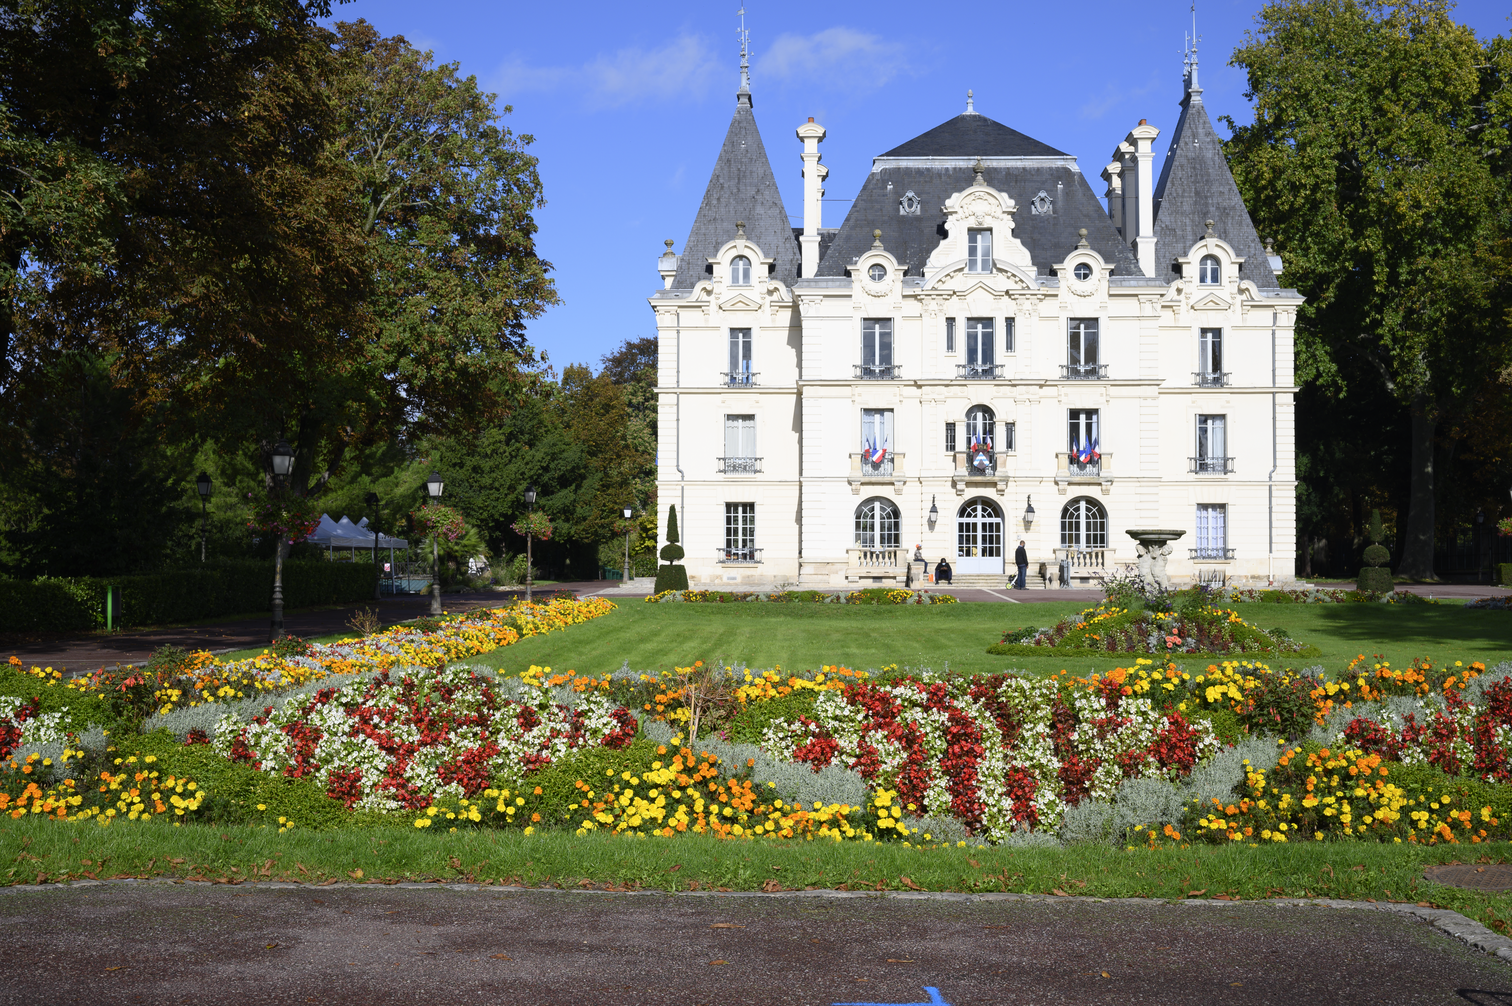
\includegraphics[width=.25\linewidth]{../assets/1512x1006/castle_bg.png}}   &
      \fbox{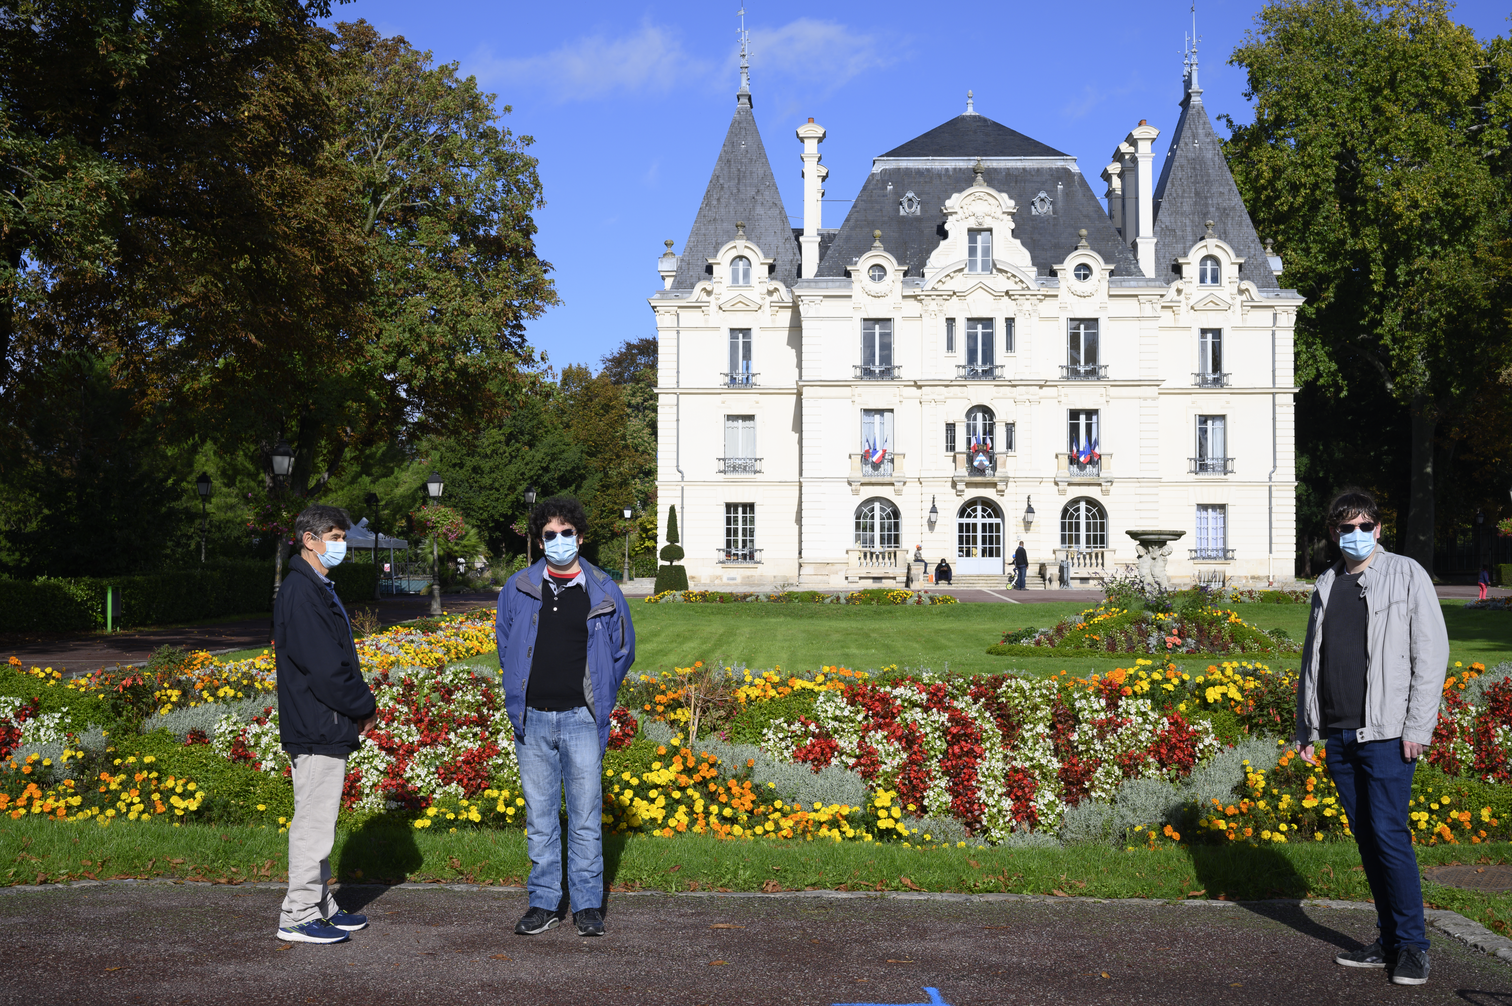
\includegraphics[width=.25\linewidth]{../assets/1512x1006/castle_fg_1.png}} &
      \fbox{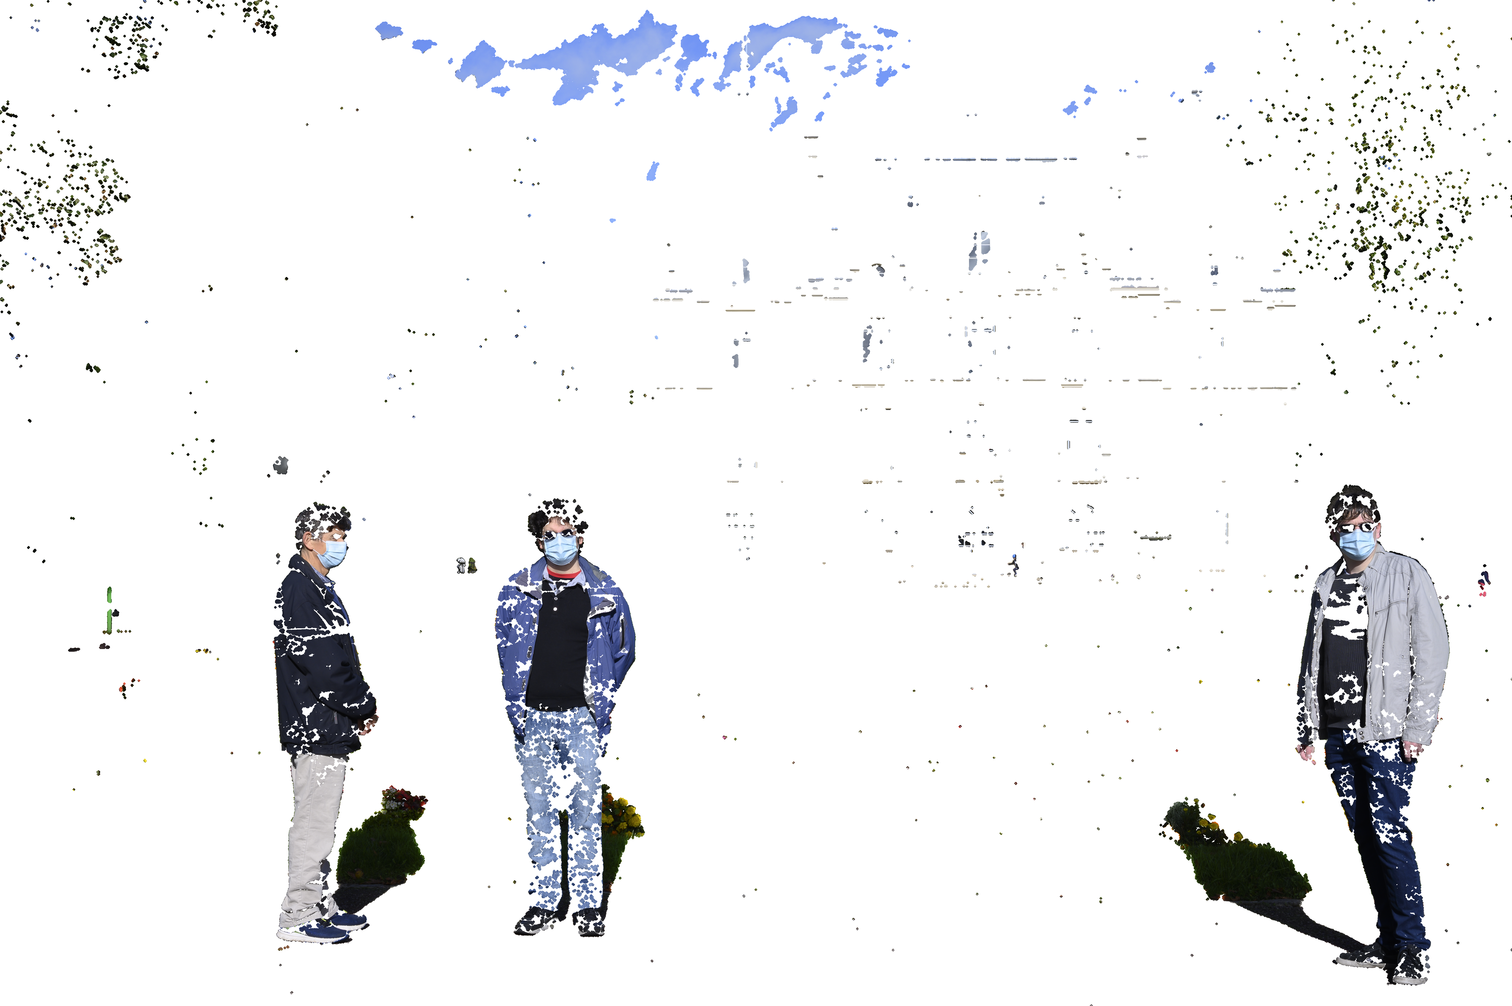
\includegraphics[width=.25\linewidth]{../assets/1512x1006/results_sig1_win5/castle/result_detected_castle_fg_1.png}} \\[5pt]
      \fbox{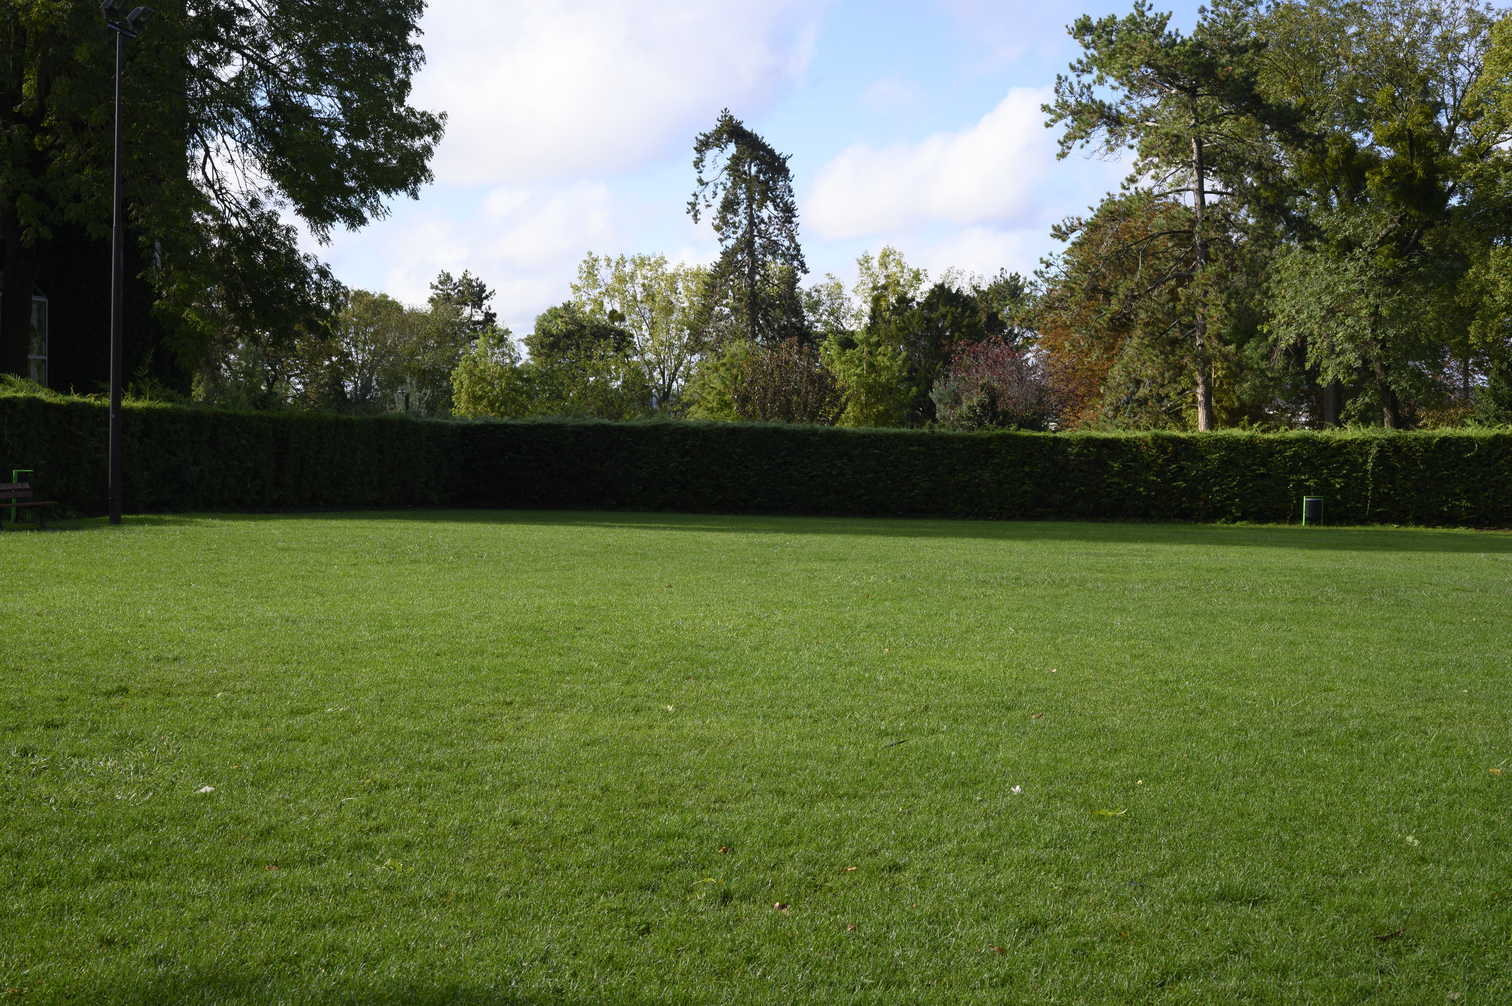
\includegraphics[width=.25\linewidth]{../assets/1512x1006/garden_bg.png}}   &
      \fbox{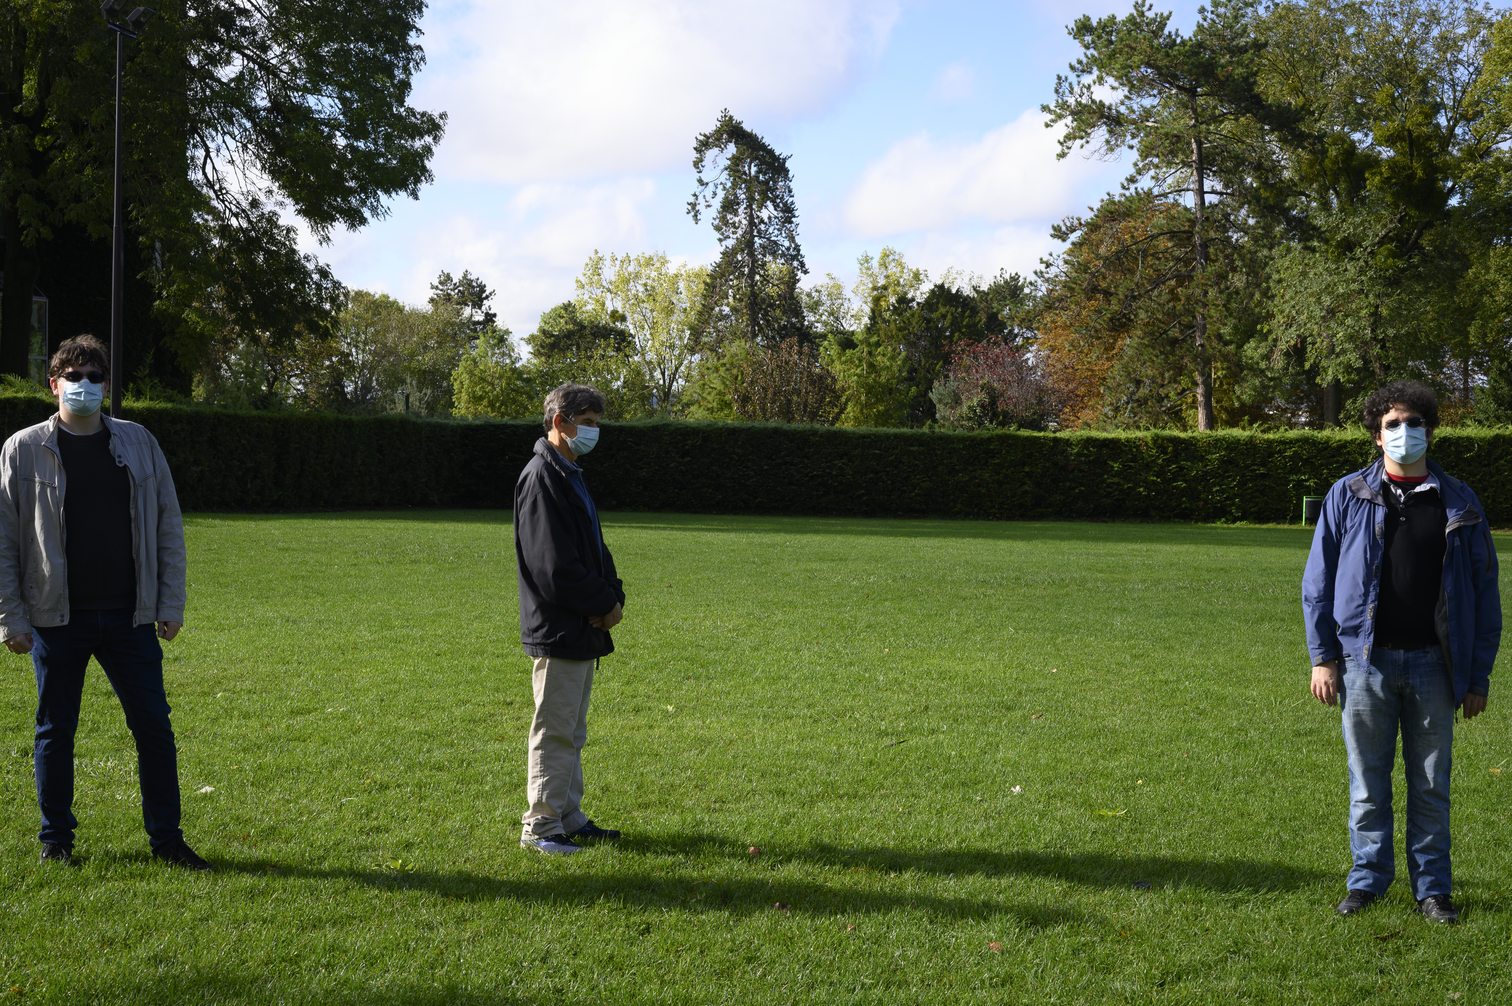
\includegraphics[width=.25\linewidth]{../assets/1512x1006/garden_fg_1.png}} &
      \fbox{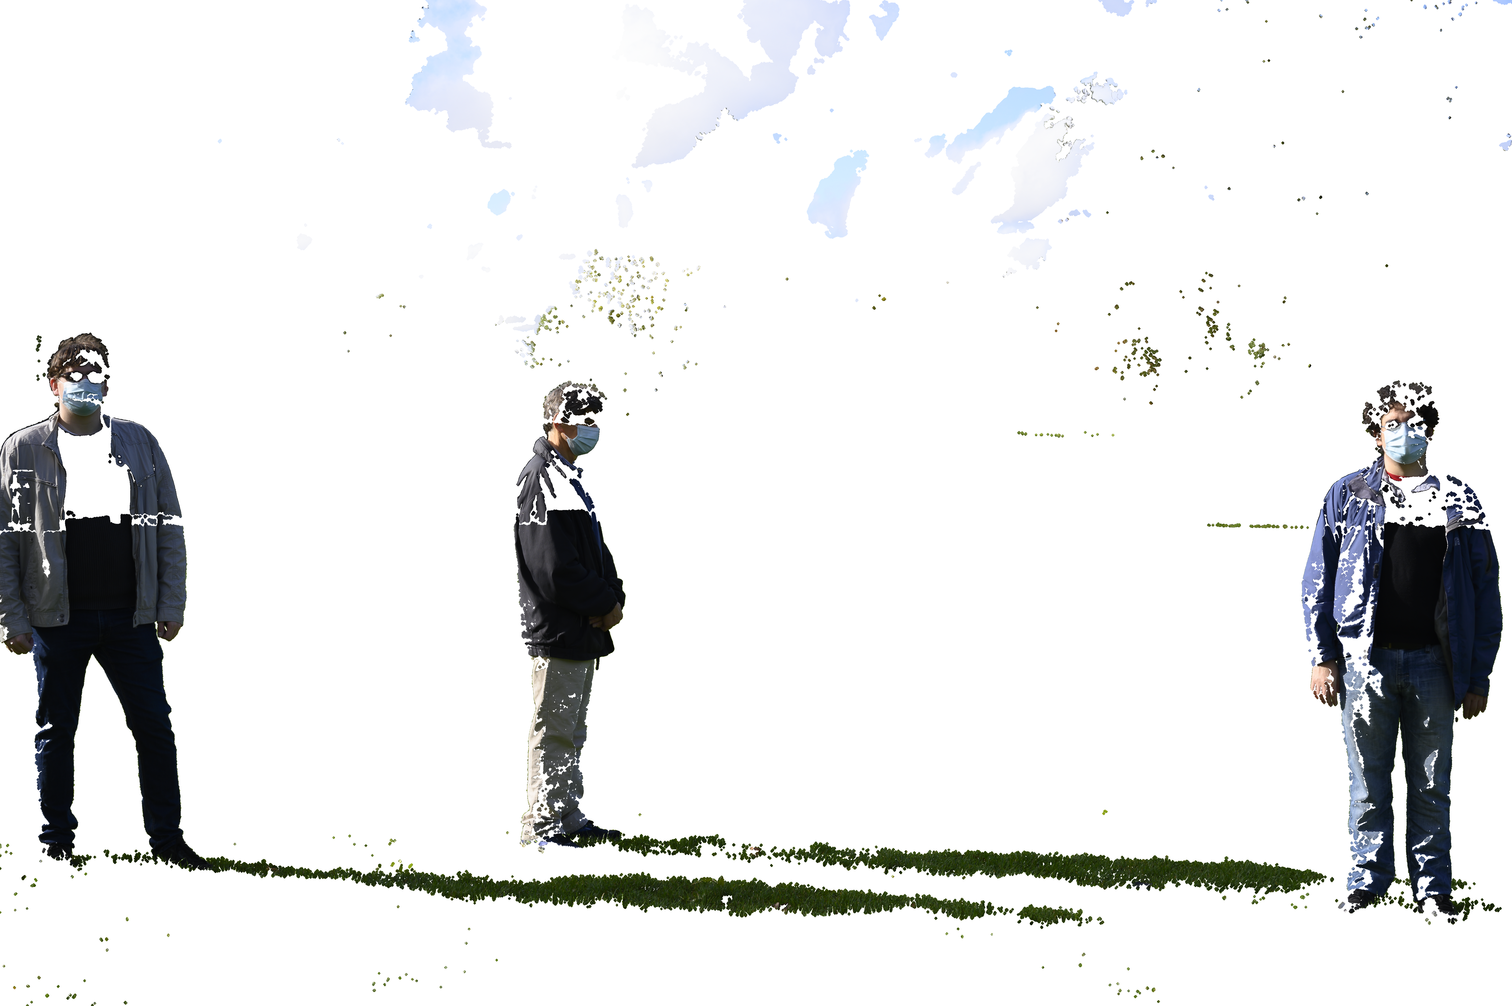
\includegraphics[width=.25\linewidth]{../assets/1512x1006/results_sig1_win5/garden/result_detected_garden_fg_1.png}}
    \end{tabular}

    \caption{Background detection: data set samples.}
    \label{fig:bg_sub.dataset_samples}
  \end{figure}
\end{frame}

\newcommand{\mystd}[1]{{\itshape(\(\pm\) #1)}}
\newcommand{\mydelta}[1]{{\itshape\bfseries #1\%}}

\begin{frame}[fragile]{Background subtraction concrete code}
  \begin{figure}
    \begin{minted}[highlightlines={3-4,6,8},highlightcolor=thistle]{c++}
    float kThreshold = 150; float kVSigma = 10;
    float kHSigma = 10;  int kOpeningRadius = 32;
    auto img_gray = view::transform(img_color, to_gray);
    auto bg_gray  = view::transform(bg_color, to_gray);
    auto bg_blurred = gaussian2d(bg_gray,  kHSigma, kVSigma);
    auto tmp_gray = img_gray - bg_blurred;
    auto thresholdf = [](auto x) { return x < kThreshold; };
    auto tmp_bin = view::transform(tmp_gray, thresholdf);
    auto ero = erosion(tmp_bin, disc(kOpeningRadius));
    dilation(ero, disc(kOpeningRadius), output);
    \end{minted}
    \caption{Pipeline implementation with \colorbox{thistle}{\emph{views}}. Highlighted code uses \emph{views} by
      prefixing operators with the namespace \texttt{view}.}
    \label{fig:view.comp.sub_bg.view_code}
  \end{figure}
\end{frame}

\begin{frame}[fragile]{Background subtraction benchmark result}
  \begin{table}
    \centering
    \begin{tabular}{l|ccc}
      \toprule
      Framework          & Compute Time            & Memory usage & \(\Delta{}\)Memory usage \\ \midrule
      Pylene (w/o views) & \(2.11s\) \mystd{144ms} & 106 MB       & \mydelta{+0}             \\
      OpenCV             & \(2.41s\) \mystd{134ms} & 59 MB        & \mydelta{-44}            \\
      Pylene (views)     & \(2.13s\) \mystd{164ms} & 51 MB        & \mydelta{-52}            \\
      \bottomrule
    \end{tabular}
    \caption{Benchmarks of the previous pipeline on a dataset (12 images) of 10MPix images. Average
      computation time and memory usage of implementations with/without \emph{views} and with OpenCV as a baseline.}
    \label{table:views.perf}
    %\vspace{-1em}
  \end{table}
\end{frame}

\begin{frame}[fragile]{Genericity limitations: C++ templates in the dynamic world}
  \begin{itemize}
    \item Static templates does not mix well with dynamic code (such as Python).
    \item Templates belong to the static world (compiled once)
    \item Python belongs to the dynamic world (interpreted multiple time)
    \item Specific work is needed to make our library available for Python.
  \end{itemize}
\end{frame}

%
%
%
\section{General Conclusion \& Perspective}

\begin{frame}{Our Hybrid solution}
  \begin{alertblock}{Hybrid solution}
    \begin{itemize}
      \item Provide type-erased interface to the static-world.
      \item Dispatch to the most efficient algorithm (precompiled) depending on type information.
      \item Allow foreign type injection.
    \end{itemize}
  \end{alertblock}
  \begin{alertblock}{Limitations}
    \begin{itemize}
      \item Code bloat.
      \item Foreign type injection is costly in performance.
      \item Still experimental.
    \end{itemize}
  \end{alertblock}
\end{frame}

\begin{frame}{Perspective: JIT}
  \begin{alertblock}{JIT infrastructure for C++/Python}
    \begin{itemize}
      \item Cython: transpile Python code into C code (for foreign type injection).
      \item AutoWIG/Cppyy: python binding generators relying on LLVM infrastructure.
      \item Xeus-cling: ready-to-use Jupyter kernel for C++.
    \end{itemize}
  \end{alertblock}
  All these existing framework can be leveraged to devise a better solution (more versatile, efficient and generic) in
  order to provide Python bindings for Pylene.
\end{frame}

\begin{frame}{Conclusion}
  \begin{itemize}
    \item We have shown the progress in generic programming in C++20 and how it serves our purpose.
    \item We have designed a Concept framework for Image Processing leveraging these progresses to write an \emph{easy to
            use}, \emph{efficient} and \emph{generic} Image processing library: \textbf{Pylene}.
    \item We have show-case a new abstraction layer: \emph{Image Views}, that are fully-fledged image type embedding Image
          Processing algorithm.
    \item We have explored way to provide those tools to the dynamic world via a static-dynamic bridge, which will be
          researched further in the future.
  \end{itemize}
\end{frame}

\begin{frame}[allowframebreaks]{Publications}
  \footnotesize
  \begin{itemize}
    \item \fullcite{roynard.2019.rrpr}
    \item \fullcite{roynard.2022.gpce}
  \end{itemize}
\end{frame}

{\setbeamercolor{palette primary}{fg=black, bg=lightgray}
\begin{frame}[standout]
  Thanks for listening!\\
  Any question?
\end{frame}
}

\maketitle

\appendix

\begin{frame}[allowframebreaks]{References}
  \printbibliography[heading=none]
\end{frame}

%\begin{frame}[fragile]{Backup slides}
%  Sometimes, it is useful to add slides at the end of your presentation to
%  refer to during audience questions.
%
%  The best way to do this is to include the \verb|appendixnumberbeamer|
%  package in your preamble and call \verb|\appendix| before your backup slides.
%
%  \themename will automatically turn off slide numbering and progress bars for
%  slides in the appendix.
%\end{frame}

\begin{frame}[fragile]{Efficient way to traverse an image}
  Introducing segmented ranges (cf. issues std::mdspan)
  \begin{columns}[T,onlytextwidth]
    \column{0.50\textwidth}
    \begin{figure}
      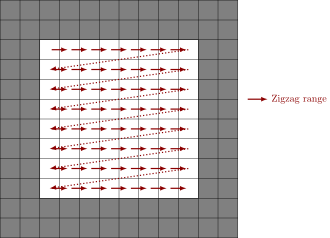
\includegraphics[width=0.8\textwidth]{../figures/linear_rng}
      \caption{Range-v3's ranges}
    \end{figure}

    \column{0.50\textwidth}
    \begin{figure}
      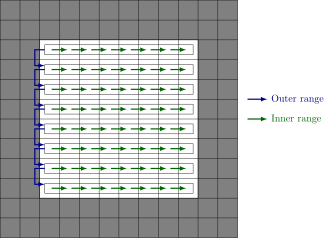
\includegraphics[width=0.8\textwidth]{../figures/segmented_rng}
      \caption{Segmented ranges}
    \end{figure}
  \end{columns}
\end{frame}

\begin{frame}[fragile]{Efficient way to traverse an image}
  Compiler needs explicit contiguous dimension in code to generate vectorized instructions.
  \begin{columns}[T,onlytextwidth]
    \column{0.50\textwidth}
    Milena's algorithm (unvectorized):
    \begin{minted}{C++}
template<class I, class SE>
mln_concrete(I) dilate(const I& f, const SE& se)
{
  mln_concrete(I) g;
  initialize(g, f);
  mln_piter(I) p(f.domain());
  mln_qiter(SE) q(se, p);
  for_all(p) // for all p in f domain
  {
    mln_value(I) v = f(p);
    for_all(q) // for all q in se(p)
      if(f.has(q) and f(q) > v)
        v = f(q);
    g(p) = v;
  }
  return g;
}
    \end{minted}
    \column{0.50\textwidth}

  \end{columns}
\end{frame}

\begin{frame}[fragile]{Efficient way to traverse an image}
  Compiler needs explicit contiguous dimension in code to generate vectorized instructions.
  \begin{columns}[T,onlytextwidth]
    \column{0.50\textwidth}
    Unvectorized algorithm:
    \begin{minted}{C++}
template<class I, , class SE>
auto dilate(I input, const SE& se) {
  auto output = input.concretize(); // clone image
  for(auto [in_px, out_px] :
        view::zip(f.pixels(), g.pixels()))
  {
    out_px.val() = out_px.val();
    for(auto nhx : se(in_px))
      out_pix.val() =
        std::max(nhx.val(), out_px.val());
  }
  return output;
}
    \end{minted}
    \column{0.50\textwidth}
    Vectorized algorithm:
    \begin{minted}[highlightlines={7-10},highlightcolor=yellow!60!white]{C++}
template<class I, class SE>
auto dilate(I input, const SE& se) {
  auto output = input.concretize(); // clone image
  // this line is needed to avoid dangling reference
  auto zipped_pixels =
        view::zip(input.pixels(), output.pixels());
  // unroll the contiguous segments
  for(auto&& row : ranges::rows(zipped_pixels))
    // optimized traversing of the segment
    for(auto [in_px, out_px] : row) {
      out_px.val() = out_px.val();
      for(auto nhx : se(in_px))
        out_pix.val() =
          std::max(in_px.val(), out_px.val());
    }
  return output;
}
    \end{minted}
  \end{columns}
\end{frame}


\begin{frame}[fragile]{Concept formal definition}
  \small
  \begin{table}[htbp]
    \begin{scriptsize}
      \begin{tabular}{l|l|l|l|}
        \cline{2-4}
                                                     & \thead{Definition }               &
        \thead{Description}                          & \thead{Requirement}                                      \\
        % Image
        \cline{1-4}
        \multicolumn{1}{|c|}{\multirow{3}{*}{Image}} & \texttt{Ima::const\_pixel\_range} & \makecell[l]{type of
          the range to iterate over
        \\ all the constant pixels} & \makecell[l]{models the concept \\
          \emph{ForwardRange}}
        \\
        \cline{2-4}
        \multicolumn{1}{|c|}{}                       & \texttt{Ima::pixel\_type}         & type of a pixel
                                                     & models the concept \emph{Pixel}                          \\
        \cline{2-4}
        \multicolumn{1}{|c|}{}                       & \texttt{Ima::value\_type}         & type of a value
                                                     & models the concept \emph{Regular}                        \\
        \cline{1-4}
        % Writable Image
        \multicolumn{1}{|c|}{\makecell[l]{Writable
        \\ Image}} & \texttt{WIma::pixel\_range} & \makecell[l]{type of the range to iterate over
        \\ all the non-constant pixels} & \makecell[l]{models the concept \\
          \emph{ForwardRange}}
        \\
        \cline{1-4}
        % StructuringElement \multicolumn{1}{|c|}{StructuringElement} &  &  & \\
        %  \cline{1-4} Decomposable \multicolumn{1}{|c|}{Decomposable} &  &  & \\
        %  \cline{1-4}
      \end{tabular}
    \end{scriptsize}
    \caption{Concepts formalization: definitions}
    \label{table:concept.definitions}
  \end{table}
  \begin{table}[htbp]
    \begin{scriptsize}
      \begin{tabular}{l|l|l|l|}
        \cline{2-4}
                                          & \thead{Expression}                              & \thead{Return Type} &
        \thead{Description}                                                                                         \\
        \cline{1-4}
        % Image
        \multicolumn{1}{|c|}{Image}       & \texttt{cima.pixels()}                          &
        \texttt{Ima::const\_pixel\_range} & \makecell[l]{returns a range of constant pixels
        \\ to iterate over it} \\
        \cline{1-4}
        % Writable Image
        \multicolumn{1}{|c|}{\makecell[l]{Writable
        \\ Image}} &\texttt{wima.pixels()} & \texttt{WIma::pixel\_range}       & \makecell[l]{returns a range of
        pixels                                                                                                      \\ to iterate over it} \\
        \cline{1-4}
      \end{tabular}
    \end{scriptsize}
    \caption{Concepts formalization: expressions}
    \label{table:concept.expressions}
  \end{table}
\end{frame}

\begin{frame}[fragile]{Pylene's views vs. Milena's morphers vs. STL ranges' views}
  \begin{alertblock}{Differences with STL ranges' views}
    \begin{itemize}
      \item STL's views are distinct from STL's containers and are constructed from ranges.
      \item Ranges are constructed from a container (and their iterators)
      \item Views is 3 levels of abstraction above a container.
    \end{itemize}
  \end{alertblock}
  \begin{alertblock}{Differences with Milena's morphers}
    \begin{itemize}
      \item Milena's morphers were not cheap to copy.
      \item Constructed from an image's reference otherwise need of deep-copy.
      \item As base image was taken by reference, possibility of dangling pointers.
      \item Dangle happens when chaining transformations with pipe (temporary copies).
      \item Const semantic (const values vs. writable values) ill-defined.
    \end{itemize}
  \end{alertblock}
\end{frame}

\begin{frame}{Static-dynamic bridge: languages type}
  \begin{figure}[htbp]
    \centering
    \includegraphics[width=.75\textwidth]{../figures/comp_inter_hybrid_summary}
    \caption{Languages types: summary diagram}
  \end{figure}
\end{frame}

\begin{frame}{Static information vs. dynamic information}
  \begin{alertblock}{Static information (known at compile-time)}
    \begin{itemize}
      \item Image's value type (unit8, rgb8, complex, etc.),
      \item Image's dimension size (1D, 2D, 3D, etc.),
      \item Architecture of the hardware hosting the program (x86, ARM, PowerPC, GPU, etc.).
    \end{itemize}
  \end{alertblock}
  \begin{alertblock}{Dynamic information (known at runtime)}
    \begin{itemize}
      \item Image's actual values,
      \item Image's actual size,
      \item Architecture of the hardware hosting the program (x86, ARM, PowerPC, GPU, etc.).
    \end{itemize}
  \end{alertblock}
\end{frame}

\end{document}